\setchapterimage[7cm]{ic/ic_icecube_crop.jpg}
\chapter{The IceCube Detector}\label{ic}
\labch{IceCube}
One\marginnote{The IceCube Laboratory, part of the \mbox{IceCube} Neutrino Observatory at the South Pole. Image credit: IceCube/NSF.} of the two most relevant instruments for this thesis is the IceCube Neutrino Observatory, a neutrino detector located at the geographic South Pole. It is the successor to the Antarctic Muon And Neutrino Detector Array (AMANDA) at the same location~\sidecite{Andres1999, Andres2000}, and has been operational for about a decade.

The basic operational principle of IceCube (and already of AMANDA) is the detection of Cherenkov light within the Antarctic ice. When charged secondary particles created by neutrino interactions travel through the ice with an energy high enough, their speed can exceed the phase velocity of light in ice, and they start to emit Cherenkov radiation. The detector consists of 5160 individual Digital Optical Modules (DOMs), buried deep in the ice, dedicated to detect this Cherenkov radiation.

\section{Cherenkov Radiation}\label{cherenkov_radiation}

Cherenkov radiation was first detected in 1934 by Soviet scientist Pavel Cherenkov~\sidecite{Cherenkov1934}. It occurs when charged particles travel within a medium with a velocity exceeding the speed of light in that very medium. The refractive index in a medium is defined as $n=\frac{c_0}{c_m}$, where $c_0$ is the speed of light in vacuum and $c_m$ is the phase velocity of light in that medium. Note that the phase velocity of light in a medium can exceed $c_0$, so $n<1$ is possible.

\begin{figure}
    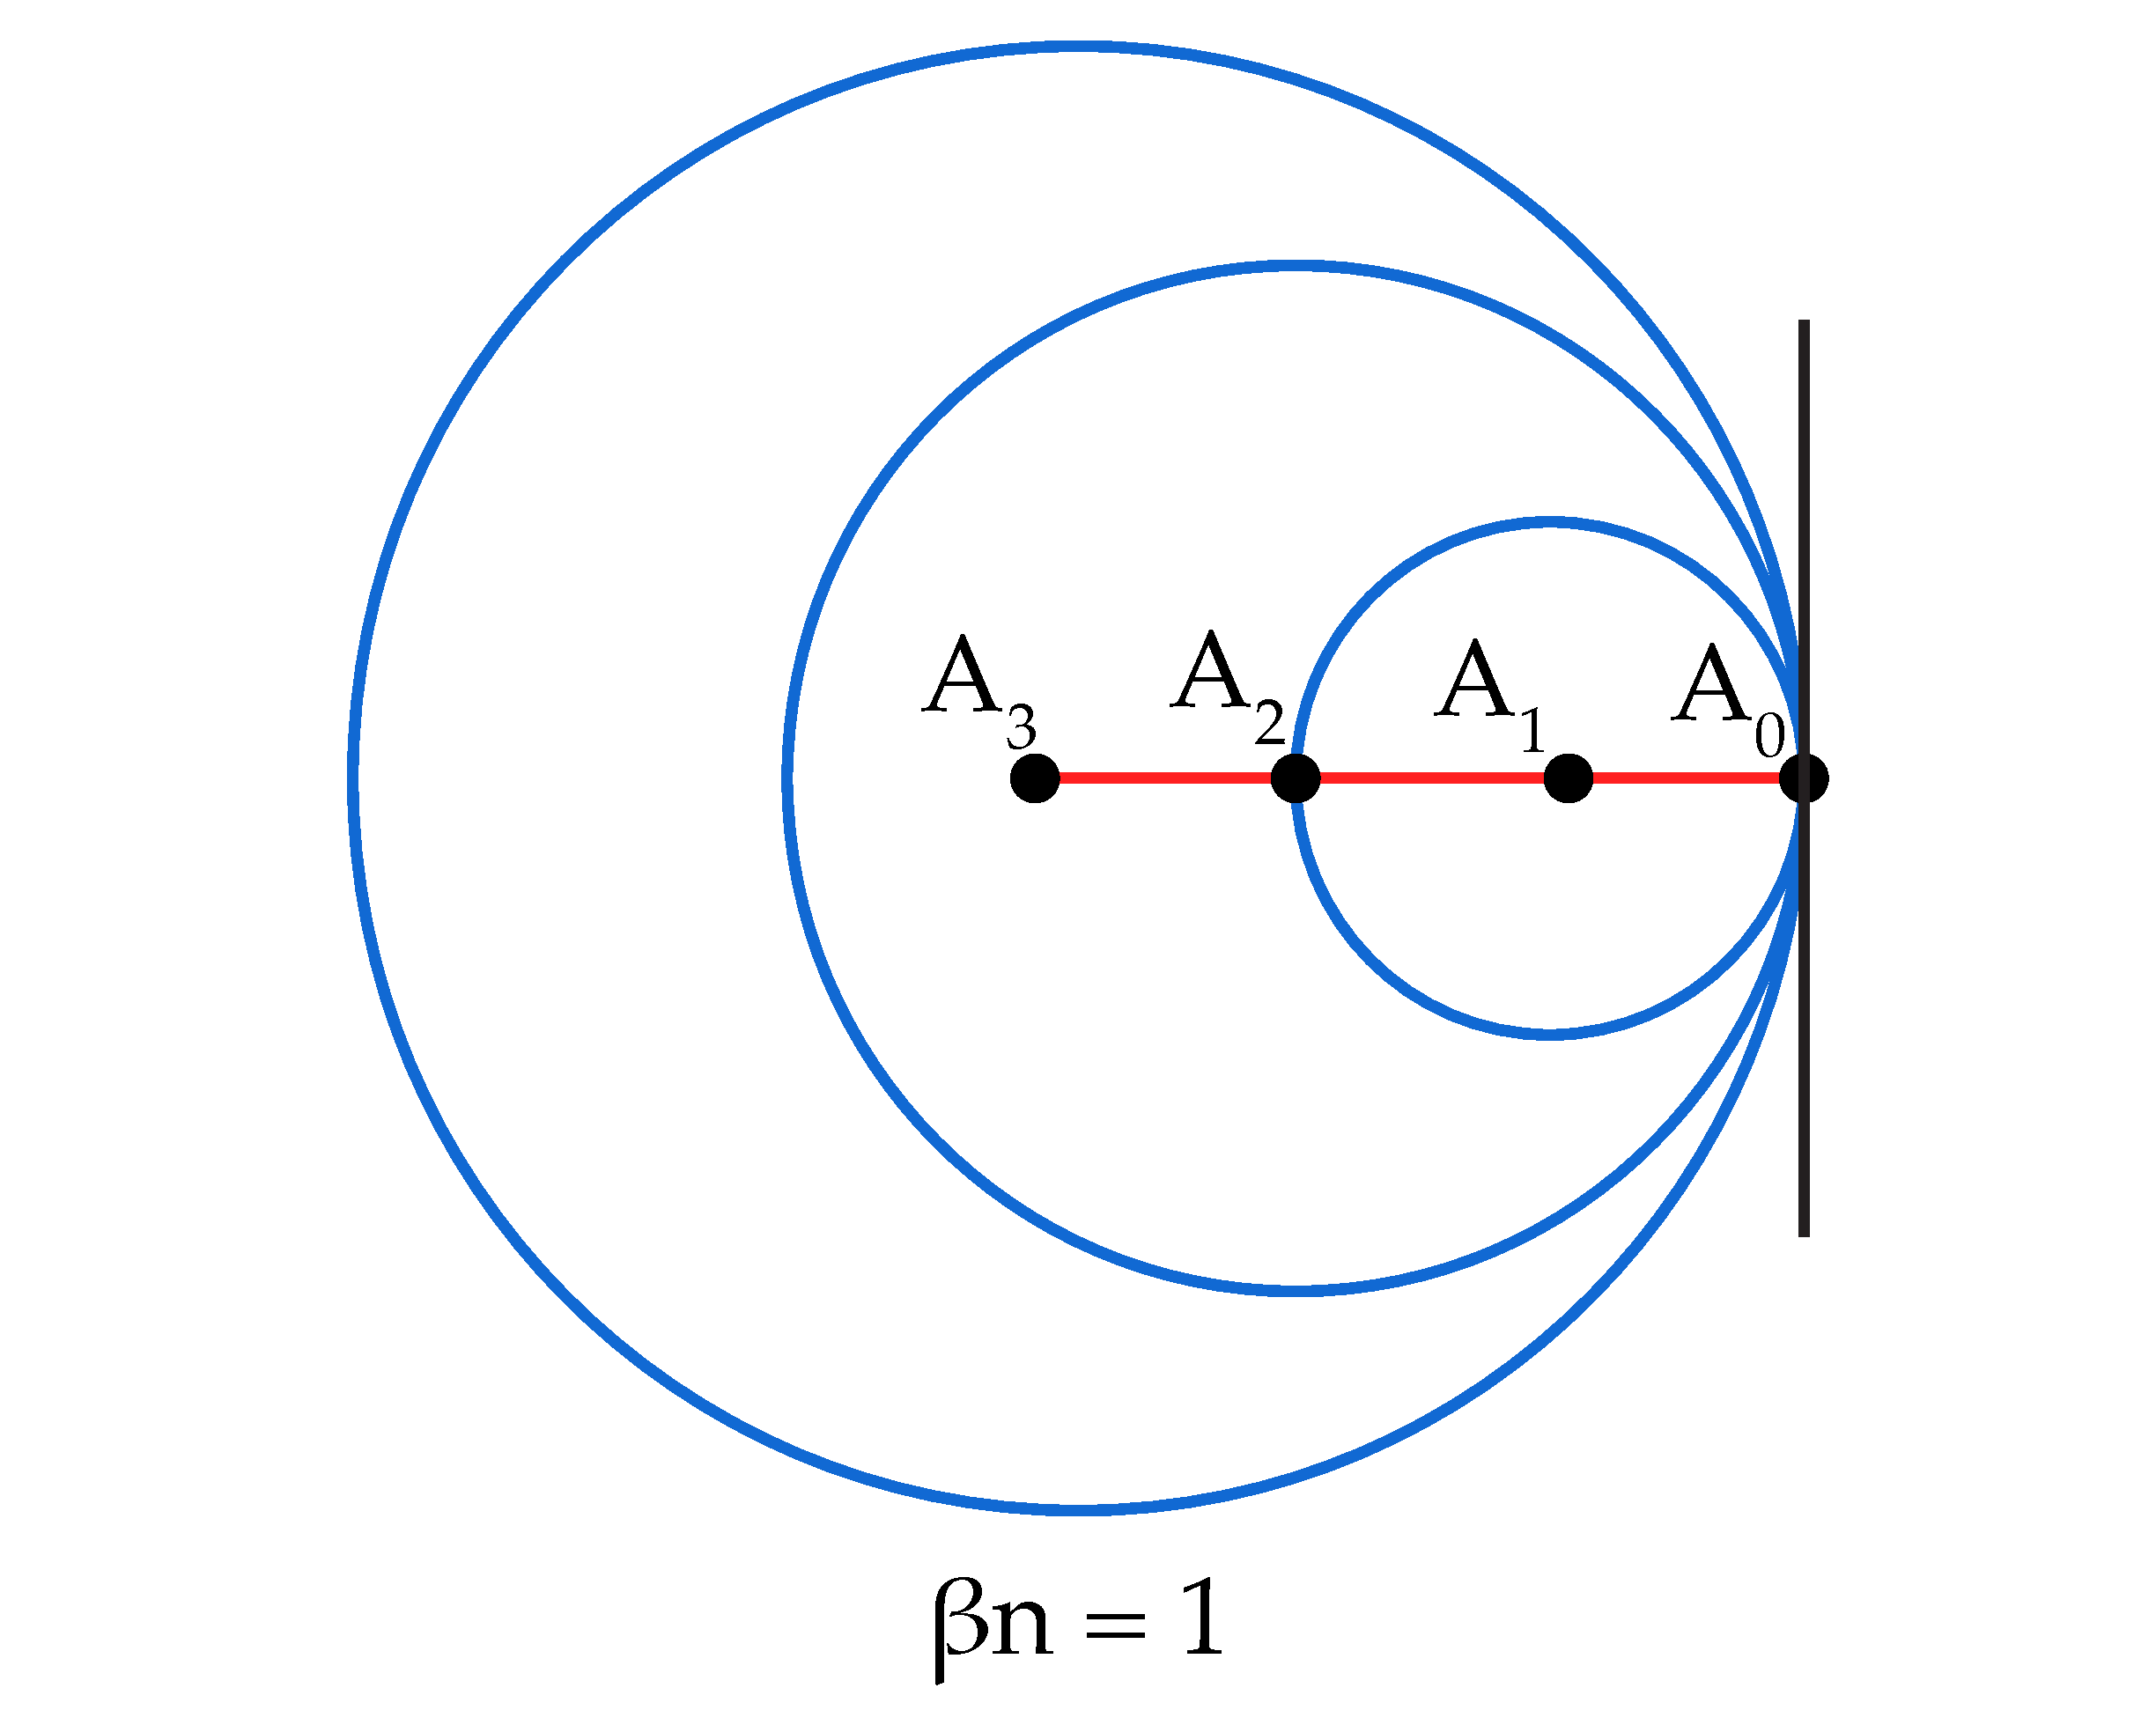
\includegraphics[width=0.49\textwidth]{ic/ic_cherenkov2.pdf}
    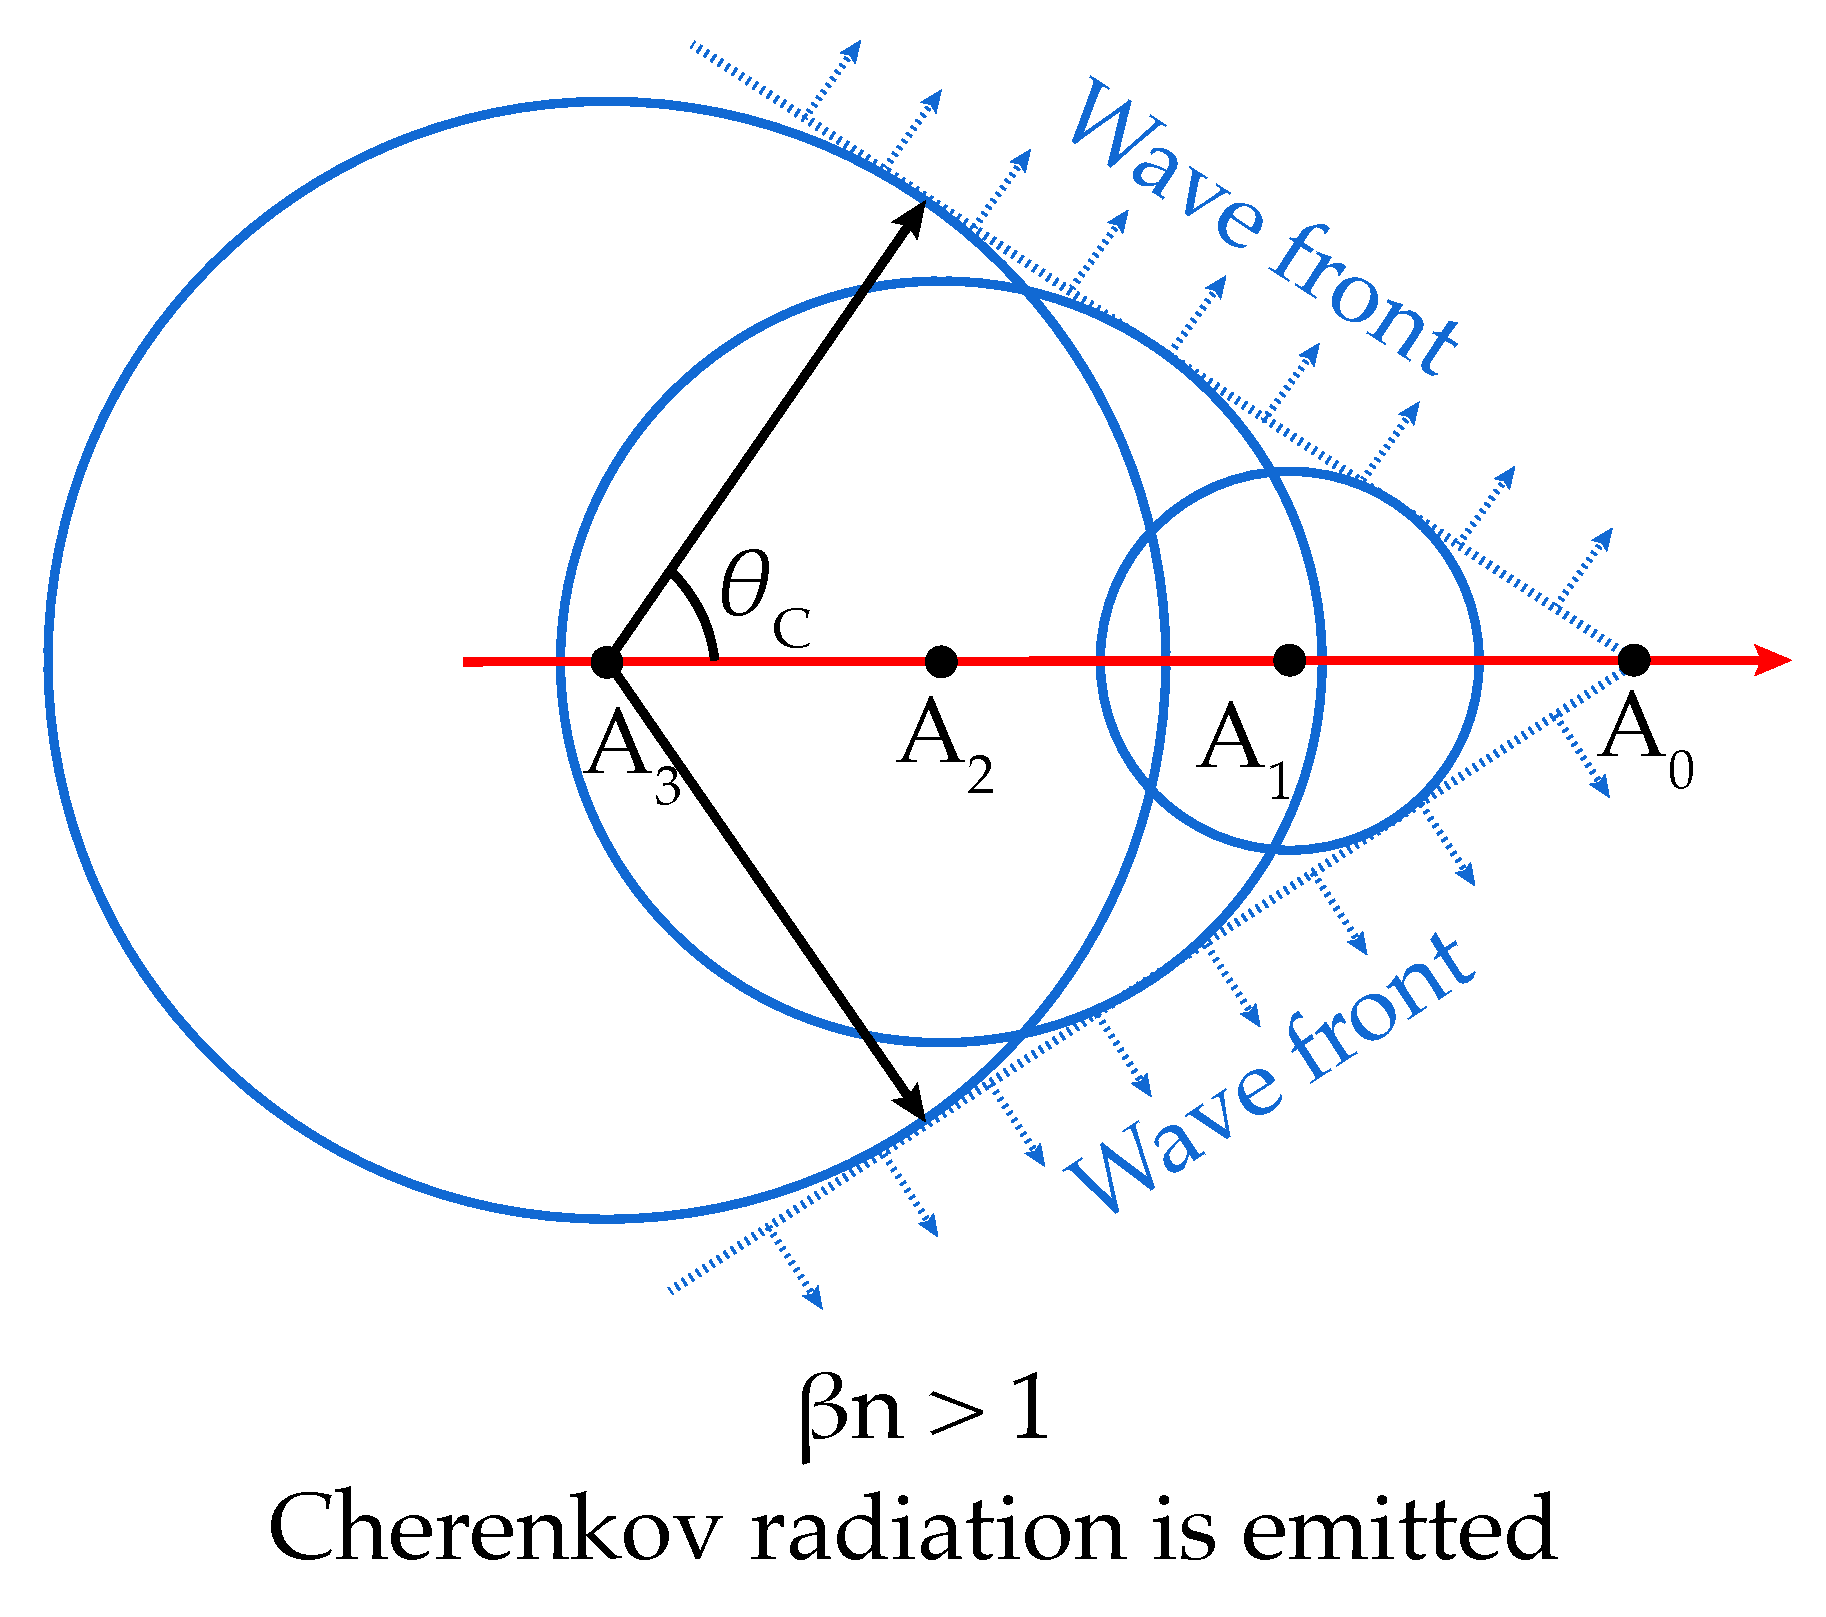
\includegraphics[width=0.49\textwidth]{ic/ic_cherenkov1.pdf}
    % \caption[Cherenkov radiation]{The principle of Cherenkov radiation. In the left figure, a particle traveling along the red path emits Cherenkov radiation at the Cherenkov angle $\theta_\text{C}$. As the radiation is emitted at different points in space and time ($\text{A}_3$ to $\text{A}_0$, radiation shown as blue circles), it forms a mutual, cone-shaped wavefront. In the figure on the right, all radiation is cancelled out by destructive interference (all circles are contained within the first one on the left, as the particle is not moving faster than light in the medium). Adapted from~\cite{LAnnunziata2020}.}
    \caption[Cherenkov radiation]{The principle of Cherenkov radiation. In the left diagram, a particle travels through a medium along the red line and is not moving faster than light within that medium. All radiation from different points in space and time ($\text{A}_3$ to $\text{A}_0$, radiation shown as blue circles) is cancelled out by destructive interference (all circles are contained within the first one on the left). Right diagram: The particle does emit Cherenkov radiation, as the different circles form a mutual, cone-shaped wavefront, radiating away at the Cherenkov angle $\theta_\text{C}$. Adapted from ~\cite{LAnnunziata2020}.}
    \labfig{cherenkov}
\end{figure}

When charged particles cross an electrically neutral dielectric medium, atoms along the particle's path are briefly polarized. When they relax back to the ground state, the atoms emit electromagnetic radiation.

For non-relativistic particles, this radiation destructively interferes with itself, canceling out all signals (left panel of Fig.~\ref{fig:cherenkov}). But if the particle is traveling faster than the speed of light within the medium $c_m$, this destructive interference does not happen. Rather, a cone-shaped wavefront gets created (right panel of Fig.~\ref{fig:cherenkov}). This wavefront constitutes Cherenkov radiation.

If the particle has speed $v=\beta c_0$, the angle $\theta$ between the particle trajectory and the direction of the Cherenkov radiation can be calculated as~\sidecite{LAnnunziata2020}

\begin{equation}
    \cos{\theta} = \frac{\beta}{n}.
\end{equation}

If the medium is ice, to first order the refractive index $n$ is $\approx1.31$.\sidenote{This assumption is rather crude. The $n$ of Antarctic glacial ice depends e.g.\ on depth; a fact we will come back to later when discussing directional reconstruction of high-energy neutrinos.} A secondary muon traveling through the ice at $0.999\,c_0$ will therefore emit Cherenkov light at an angle of $\theta = \cos^{-1}{\big(\frac{0.999}{1.31}\big)} \approx \SI{40}{\degree}$.
\begin{marginfigure}
    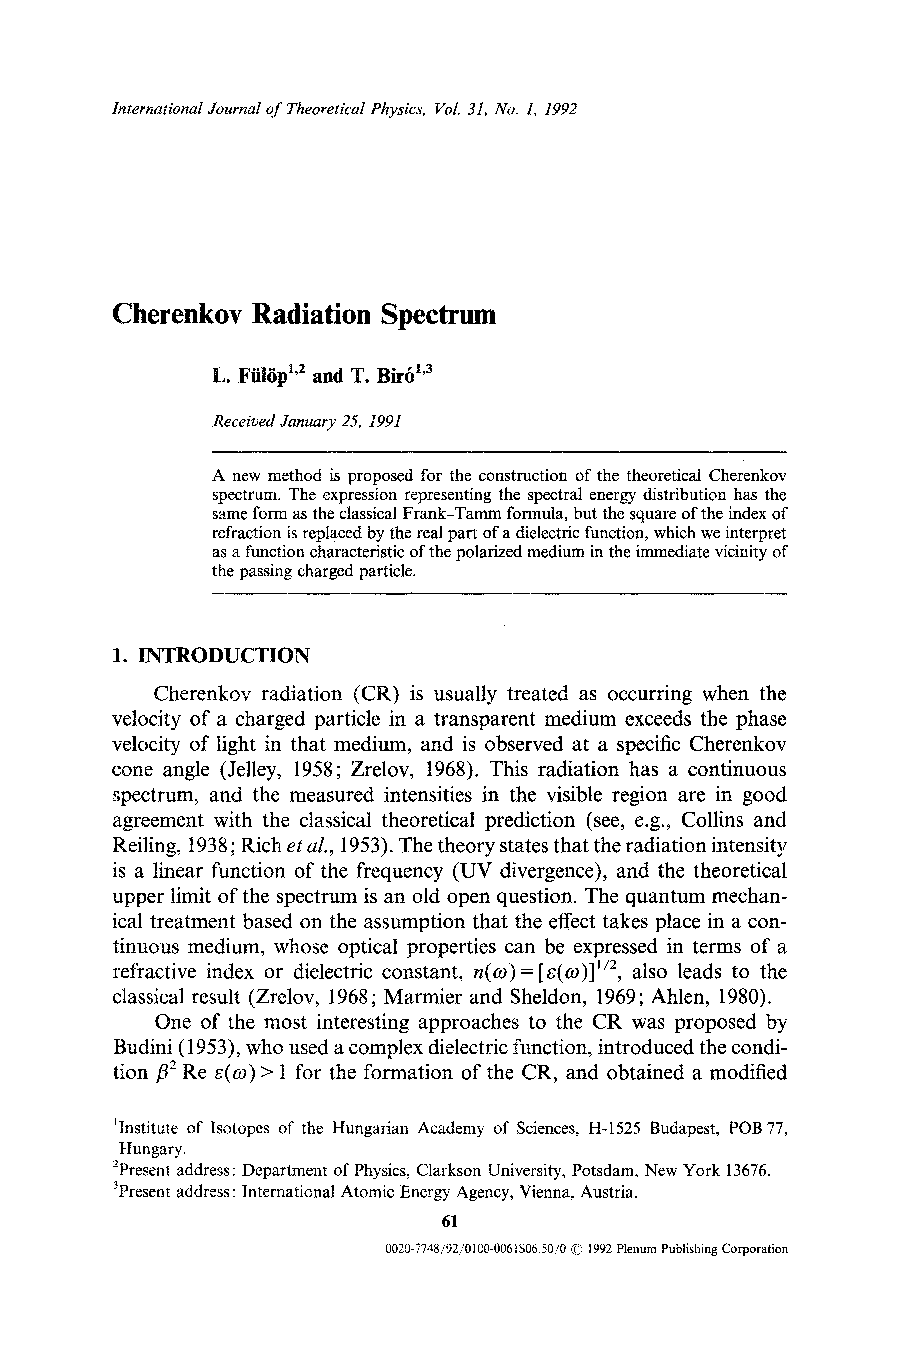
\includegraphics{ic/ic_cherenkov_spectrum.pdf}
    \caption[Cherenkov spectrum]{Cherenkov spectrum for a particle with $v=0.8 \,c_0$ in water. The intensity peaks around $\SI{4e15}{\Hz}$, corresponding to a wavelength of \SI{75}{\nm}, lying at the high-frequency end of the UV spectrum. Adapted from~\cite{Fulop1992}.}
    \labfig{cherenkov_spectrum}
\end{marginfigure}
Cherenkov radiation has a smooth spectrum, with a relative intensity roughly proportional to the frequency. The refractive index of a medium also depends on the frequency, dropping below 1 in the X-ray\todo{in ice?}. From this it follows that Cherenkov radiation appears blue to the human eye (the high-frequency part dominates) and its intensity peaks in the Ultra Violet (UV), before it sharply drops off in the X-ray regime~\sidecite{Fulop1992}, see Fig.~\ref{fig:cherenkov_spectrum}.

\section{Instrumentation}

IceCube detects neutrinos by observing the optical and UV part of their secondary particle Cherenkov spectrum with 5160 DOMs in the ice. To understand how this is done, one first needs to look at the working principle of a Photomultiplier Tube (PMT), the basic instrument within the DOMs.

\subsection{Photomultiplier Tubes}
PMTs are devices used to detect very faint light signals by amplifying them. They consist of vacuum tubes and were successfully realized for the first time in the 1930s~\sidecite{Iams1935}.

\begin{figure}[h!]
    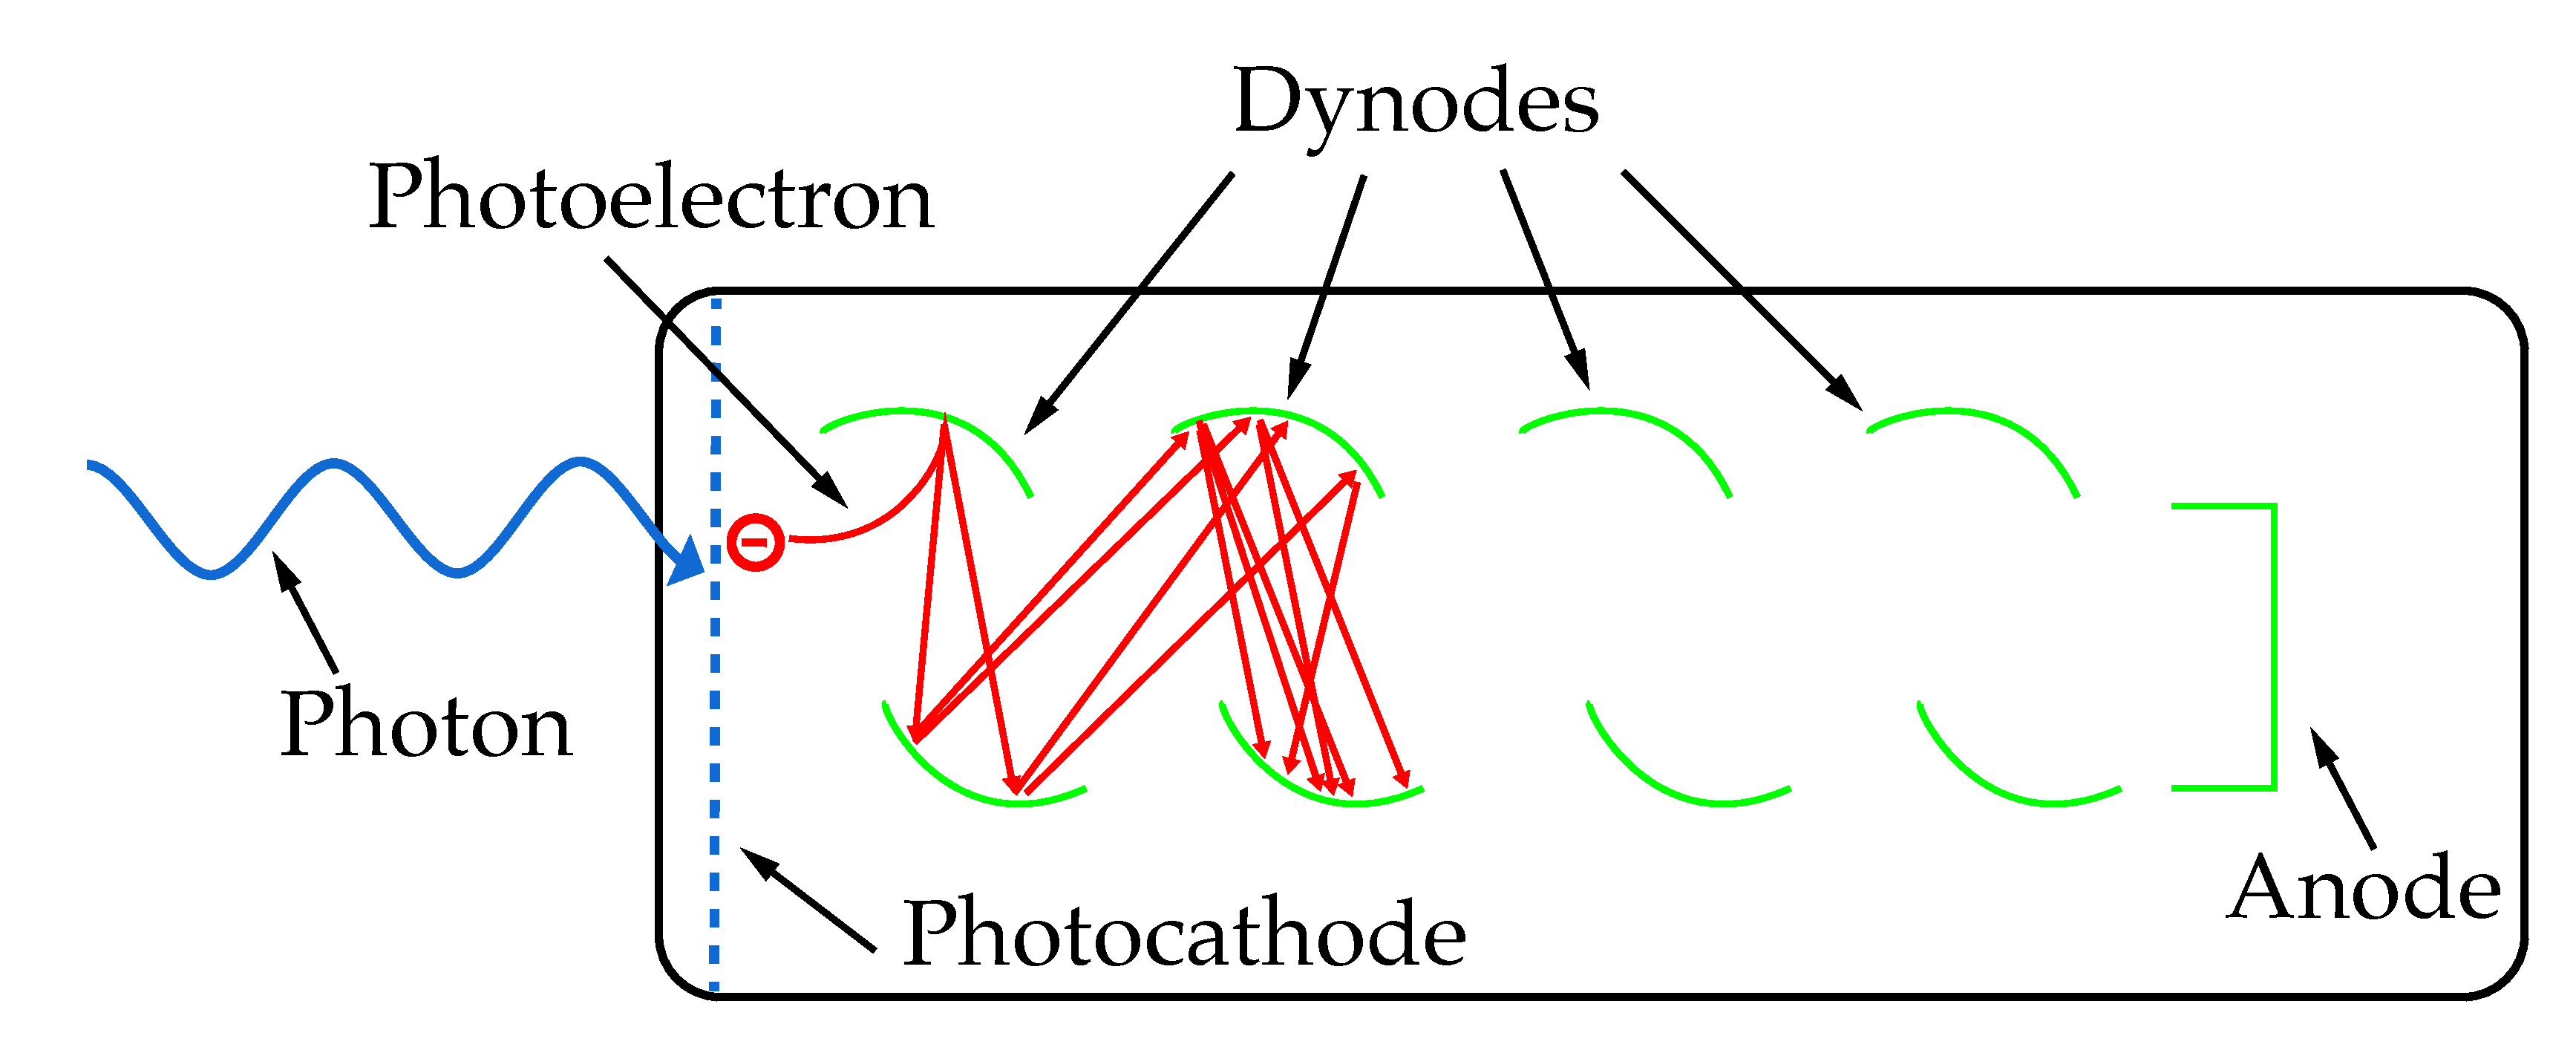
\includegraphics[width=0.8\textwidth]{ic/ic_pmt_annotated.pdf}
    \caption[PMT schematic]{A photomultiplier tube. The incident photon creates a photoelectron on the left, which gets multiplied at each dynode along the way to the anode on the left, creating an avalanche of electrons. Adapted from~\cite{Bednarski2014}.}
    \labfig{pmt}
\end{figure}

As one can see in Fig.~\ref{fig:pmt}, there are three principal components: a cathode, several dynodes and an anode. When photons hit the cathode, they can release electrons via the photoelectric effect~\sidecite{Einstein1905}. These photoelectrons are then accelerated (towards the right side in Fig.~\ref{fig:pmt}) by an electric field within the tube. This field is generated by applying a high voltage between the cathode and the anode.

To amplify the signal, a number of dynodes are placed between cathode and anode. These are additional electrodes with subsequently higher voltages. When the photoelectron hits the first dynode, a number of secondary electrons are generated, which are then accelerated towards the next dynode by the electric field. This process repeats for every dynode, generating an electron avalanche exponentially amplifying the original single photoelectron signal. The number of secondary electrons hitting the anode is proportional to the number of incident photons, resulting in a linear detector response (as long as the detector stays below its saturation limit)~\sidecite{Wright2017}.

IceCube uses PMTs made by Hamamatsu Photonics (R7081--02) and which are sensitive to photons between 300 and \SI{650}{\nm}. They have a quantum efficiency (QE) at \SI{390}{\nm} of \SI{25}{\percent}, are operated with a voltage of \SI{1500}{\V} and have a gain (electron multiplication factor) of \num{e7}. The photon-sensitive surface area is typically \SI{530}{\cm\squared}~\sidecite{Abbasi2010}.

\subsection{The Digital Optical Module}\label{DOM}
\begin{marginfigure}
    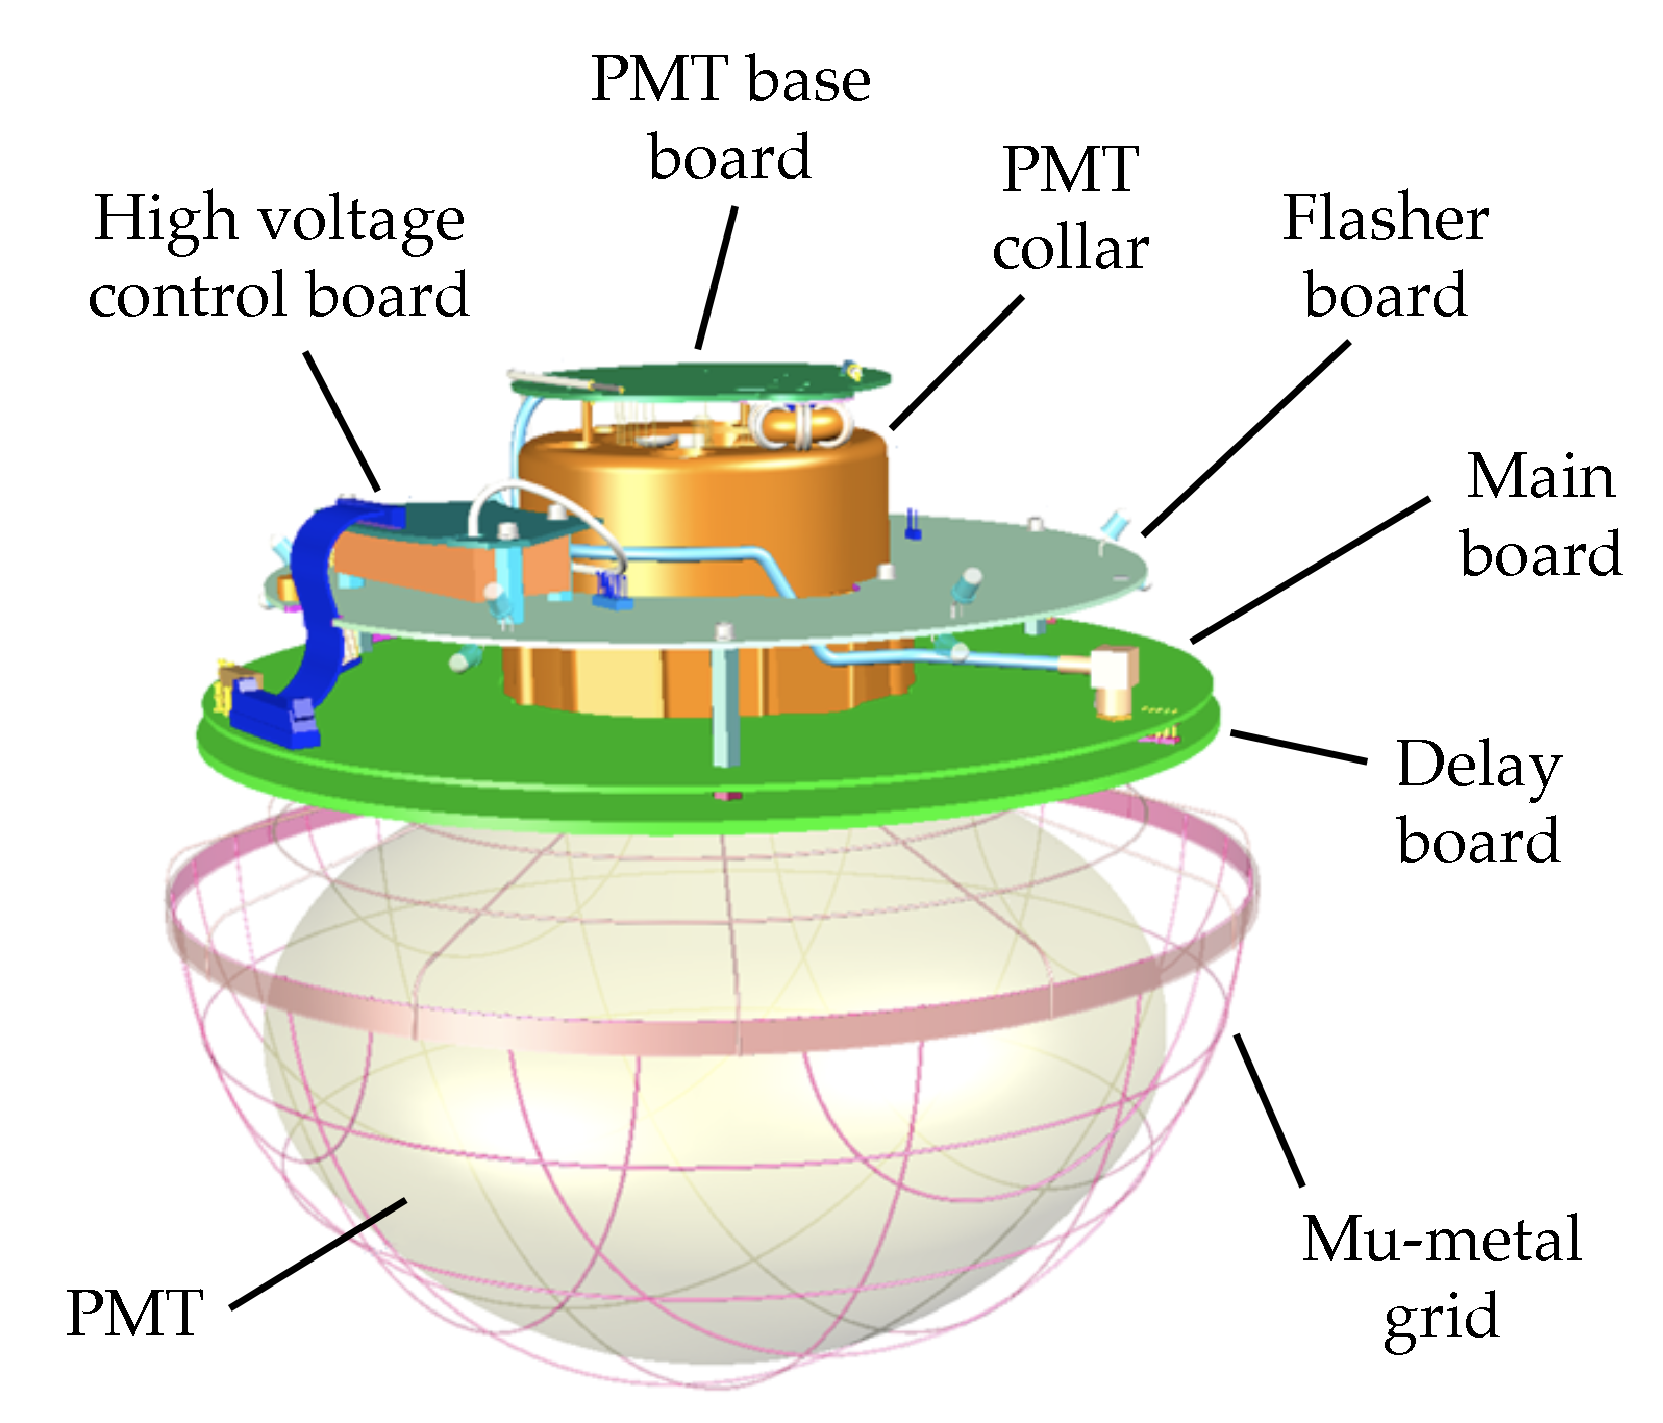
\includegraphics{ic/ic_DOM.pdf}
    \caption[IceCube digital optical module]{The IceCube DOM seen from the side. The detecting side of the PMT is facing downwards, with the main board and the PMT base board on top. From~\cite{Aartsen2017}.}
    \labfig{ic_dom}
\end{marginfigure}

The individual IceCube PMTs for detecting the Cherenkov radiation are enclosed in the DOMs. Each DOM consists of a pressure-resistant glass sphere, several controller boards and the PMT, facing downward (see Fig.~\ref{fig:ic_dom}). The glass sphere can withstand long-term pressure of \SI{250}{\bar}. The optical transmission of the spheres was measured to be \SI{93}{\percent} at \SI{400}{\nm}, decreasing to \SI{10}{\percent} at \SI{315}{\nm}.

The circular main board hosts data acquisition and control systems, as well as units for communication and a power converter. Another board, the PMT base board, interfaces with the PMT, while additional boards delay the PMT signals and generate the high voltage current powering the PMT. Additionally, there is a so-called Flasher Board that controls Light-Emitting Diodes (LEDs). These are used to generate light flashes which can be received by neighboring DOMs for calibration purposes~\sidecite{Aartsen2017}.

Because of data storage restrictions, the DOMs only record and digitize the photon signal after several trigger criteria have been met. The digitized voltage over time detected by the PMTs is called a waveform, and combined with a timestamp it comprises the basic datum in IceCube, a hit.

To fully record the waveform after a hit, the signal needs to be stored in a buffer. This is realized with the delay board, which routes the analog PMT signal through a \SI{10}{\m} long, serpentine copper trace to delay it by \SI{75}{\ns}.

When a hit is detected, the DOM sends a tag signal to the neighbor and next-to-nearest neighbor DOMs. If no neighbors detect a hit, the isolated hit will only contain the timestamp, the amplitude and charge information extracted from the waveform. When at least two neighboring DOMs also detect a hit within \SI{0.25}{\micro\s}, a Local Coincidence (LC) is triggered. If the signal passes a threshold of 0.25 photoelectrons, the recorded waveforms are digitized and appended to the hits tagged as LC~\cite{Aartsen2017}.

\begin{marginfigure}
    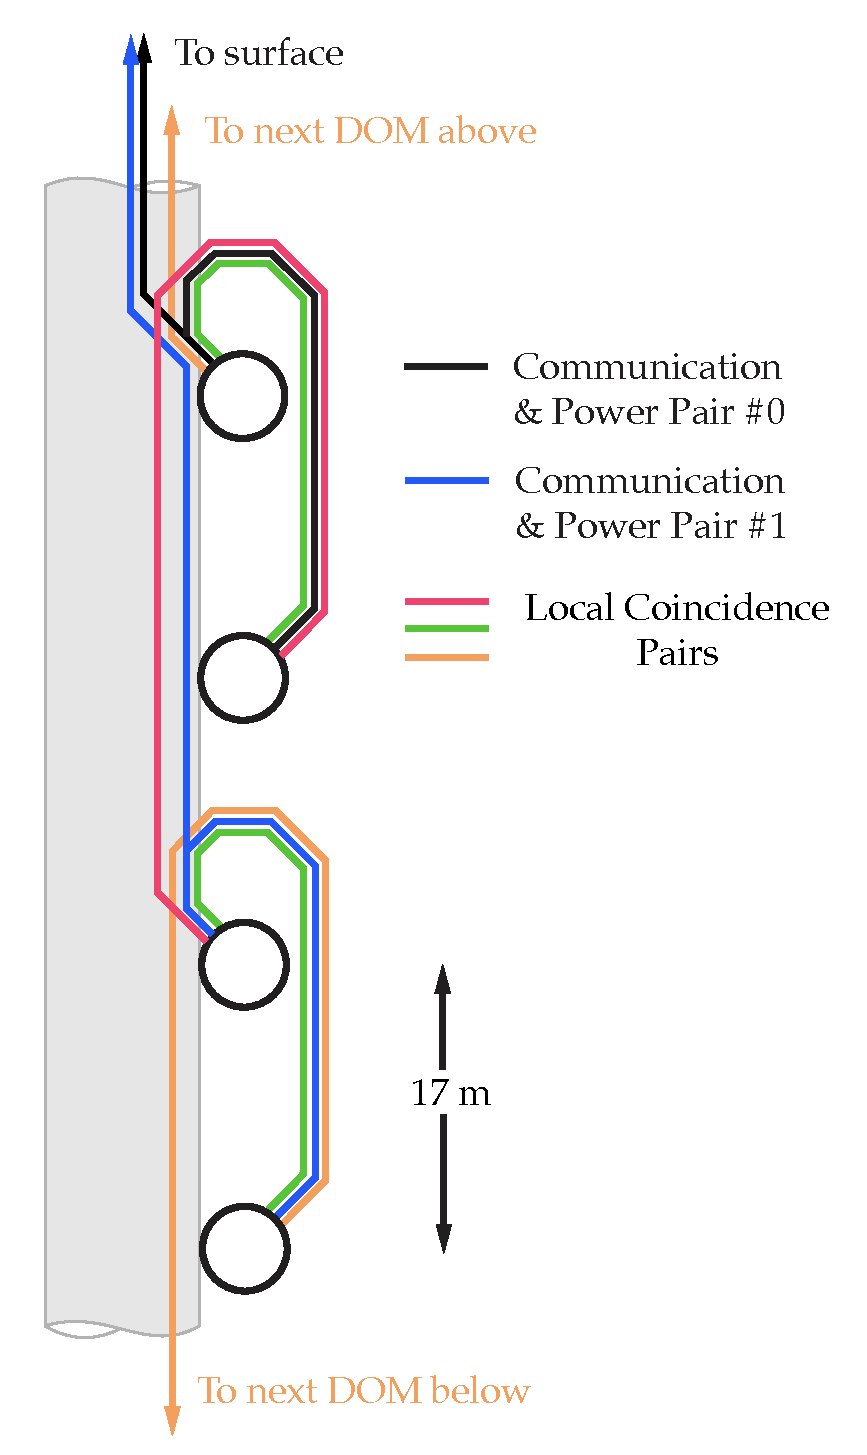
\includegraphics{ic/ic_DOM_connections.pdf}
    \caption[IceCube DOM connections]{Connection scheme for four IceCube DOMs along one string. Pairs of DOMs share one twisted-pair cable. Also, each DOM is directly connected to its direct neighbors above and below. Adapted from~\cite{Aartsen2017}.}
    \labfig{ic_dom_connections}
\end{marginfigure}

The digitization of the PMT waveform is done with the Analog Transient Waveform Digitizer (ATWD), a custom-built Application Specific Integrated Circuit (ASIC). Usually lying dormant, the ATWDs start to capture the delayed waveform when the PMT discriminator initiates it. The captured waveforms are only digitized in case a hit (i.e.\ local coincidence) is registered~\cite{Aartsen2017}.

The DOMs are connected to the IceCube Laboratory (ICL) with twisted-pair copper cables. The power for the DOM is also transmitted with this cable. Two DOMs share one twisted-pair cable, and each DOM is also directly connected to its two neighbors on the same string. Fig.~\ref{fig:ic_dom_connections} shows the connection layout.

The Flasher Board houses 12 LEDs operating at a wavelength of \SI{\sim400}{\nm}. These are used to verify the DOM timing response, to measure the DOM in-ice position, to determine the optical properties of the ice, and to verify the reconstruction algorithms~\cite{Aartsen2017}.

\subsection{Detector Layout}
In total, approximately 5800 DOM units were built and tested, 300 failing tests and the rest being delivered to the South Pole. The vast majority of these were ultimately deployed (5160 in total). The final detector layout (since the last drilling campaign 2010/2011, see below) consists of 86 strings. The DOMs were deployed along those strings, like pearls on a necklace. Each string contains 60 DOMs, with an average horizontal spacing between strings of \SI{125}{\meter}~\cite{Aartsen2017}.

The instrumented part of the strings starts at \SI{1450}{\m} below surface, with one DOM every \SI{17}{\m} to a depth of \SI{2450}{\m}, just above the bedrock at a depth of \SI{2820}{\m}. In Fig.~\ref{fig:ic_sideon} the layout of the in-ice array can be seen. The strings follow a roughly hexagonal layout (see Fig.~\ref{fig:ic_top_down}), with a side length of \SI{1}{\km\squared}. The total instrumented volume of glacial ice is thus \SI{1}{\km\cubed}~\cite{Aartsen2017}. Of the 5160 deployed DOMs, 92 are dead as of March 2023, a loss of \SI{1.7}{\percent}\sidenote{This is better than the predicted failure percentage, which was projected to be \SI{2}{\percent} by 2023~\cite{Aartsen2017}.}.

One can see in Fig.~\ref{fig:ic_top_down} that there is a region in the center of the detector which is more densely instrumented: The strings are closer to each other, and also the spacing between DOMs on these strings is reduced from \SI{17}{\m} to \SIrange{7}{10}{\m}. This part of the detector is DeepCore, designed to have a lower energy threshold of \SI{10}{\GeV}, a significant improvement over the \SI{100}{\GeV} for the rest of the detector. The DOMs within DeepCore are also modified for this goal, as they are equipped with PMTs that have a \SI{35}{\percent} higher QE compared to the `normal' DOMs~\cite{Aartsen2017}.

\begin{figure}[htbp]
    \includegraphics[width=1.\textwidth]{ic/ic_side_view_font.pdf}
    \caption[IceCube side-on]{Side view of the IceCube detector, showing the instrumented array deep in the Antarctic glacial ice. In the center on top is the IceCube Laboratory, where data processing takes place. From~\cite{Ahlers2018a}.}
    \labfig{ic_sideon}
\end{figure}

\begin{marginfigure}
    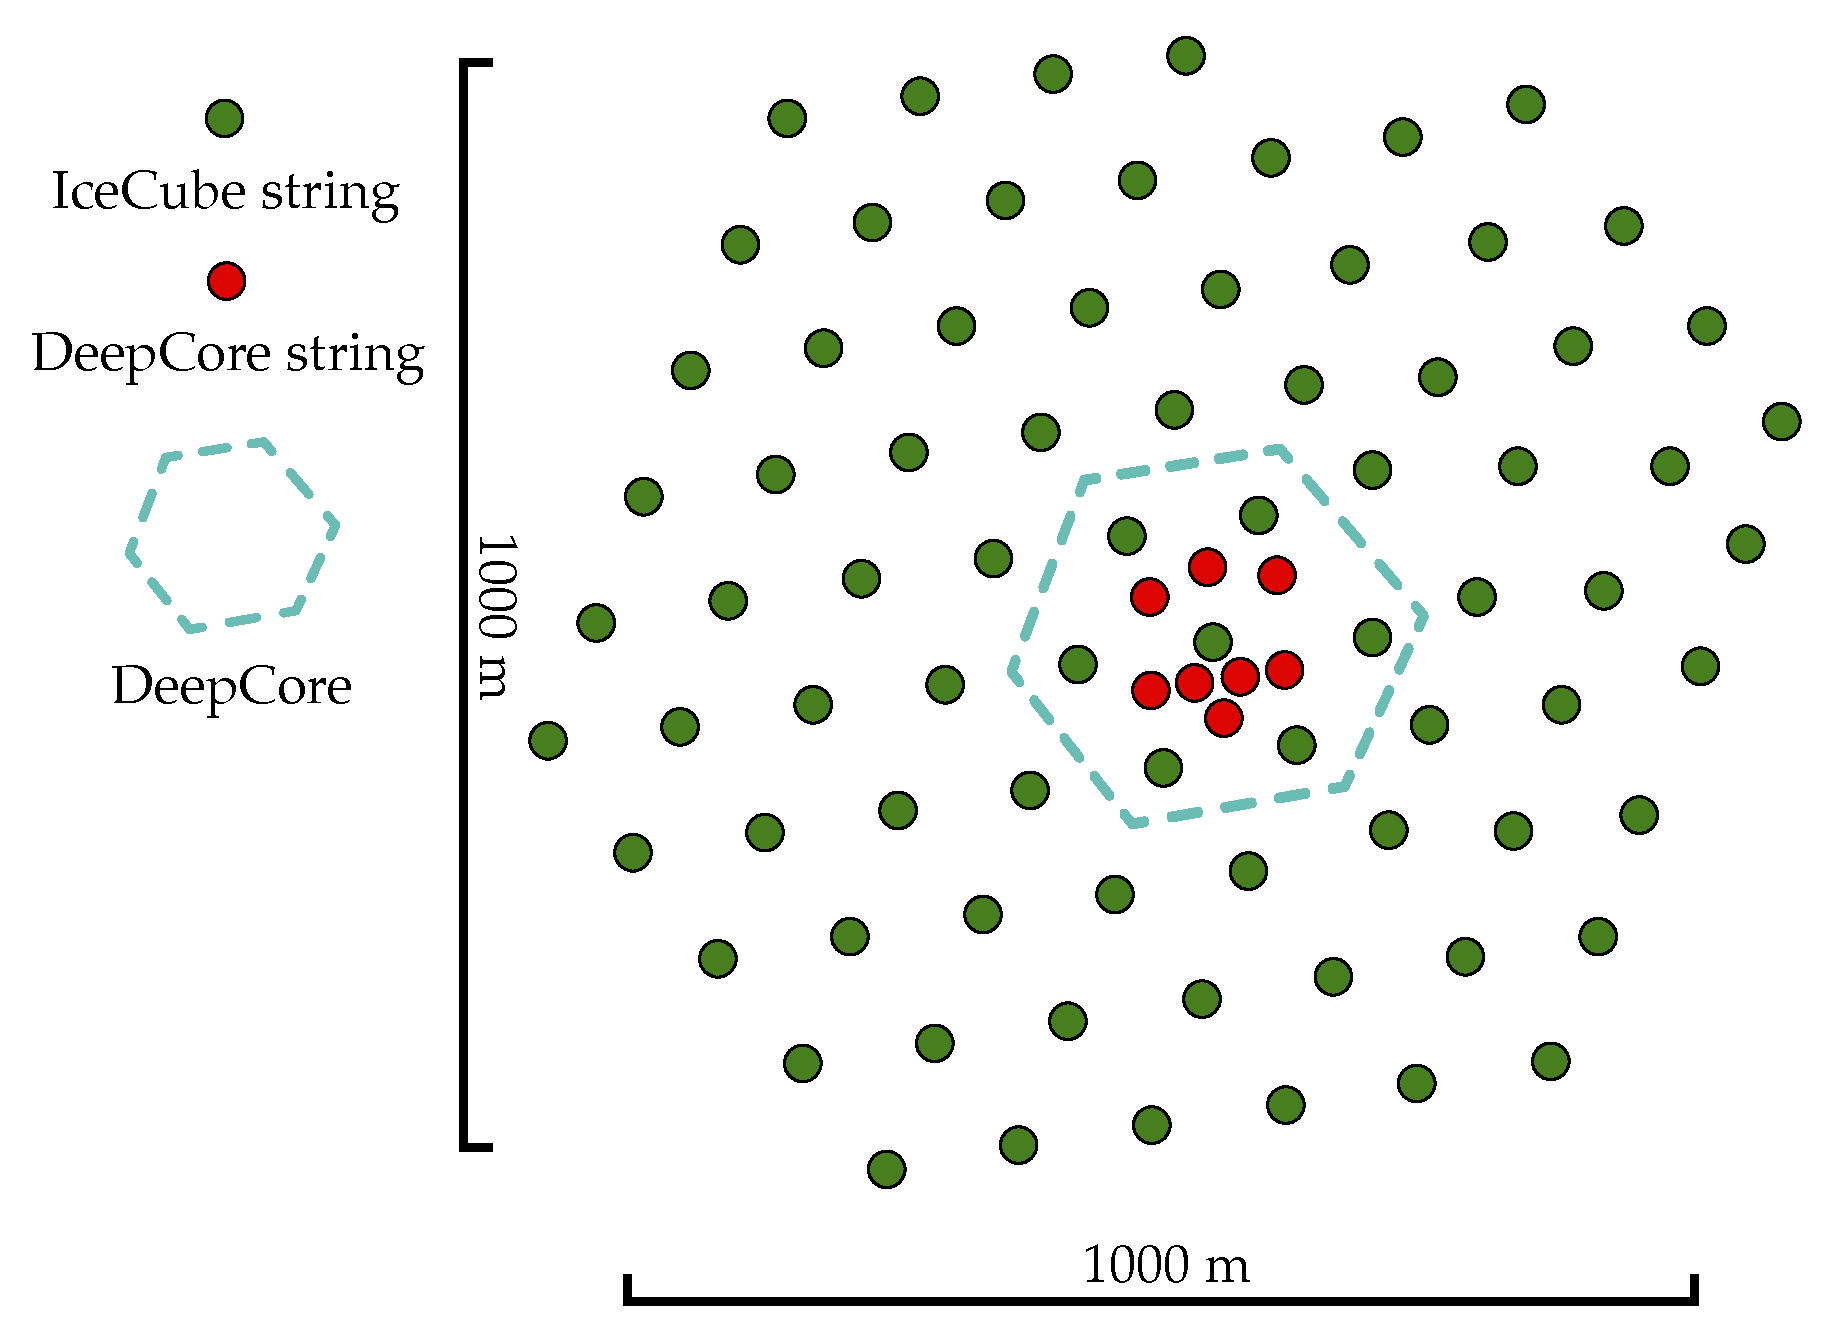
\includegraphics{ic/ic_top_view.pdf}
    \caption[IceCube top-down view]{Top-down view of the IceCube detector, spanning \SI{1}{\square\km} on the surface. From~\cite{Ahlers2018a}.}
    \labfig{ic_top_down}
\end{marginfigure}

\subsection{Deployment}

As one can imagine, embedding the DOMs within the ice was a highly non-trivial task. It required drilling 86 boreholes with a diameter\sidenote{The hole diameter was larger than the DOM diameter (\SI{35}{\cm}) to account for partial refreezing of the borehole.} of roughly \SI{60}{\cm} and a length of \SI{2500}{\m}. This was achieved over several drilling campaigns with the Enhanced Hot Water Drill (EHWD) specifically built for this task. This drill had a total power of \SI{5}{\mega\W} and was able to drill with a maximum speed of \SI{2.2}{\meter\per\minute}. With these performance characteristics, one hole was drilled every \SI{48}{\hour} on average, with drill operations round the clock~\cite{Aartsen2017}. It took seven drilling seasons to deploy the final IceCube86 setup, from the Antarctic summers 2004/2005 to 2010/2011. Fig.~\ref{fig:ic_drill} shows the tower operations site directly above the borehole~\sidecite{Benson2014}.

The water for drilling the holes was heated to \SI{88}{\celsius} with 35 water heaters working in parallel, each providing \SI{125}{\kilo\W} power. The average amount of fuel used per drill hole was \SI{27000}{\liter}~\cite{Benson2014}.

\begin{figure}[hbtp]
    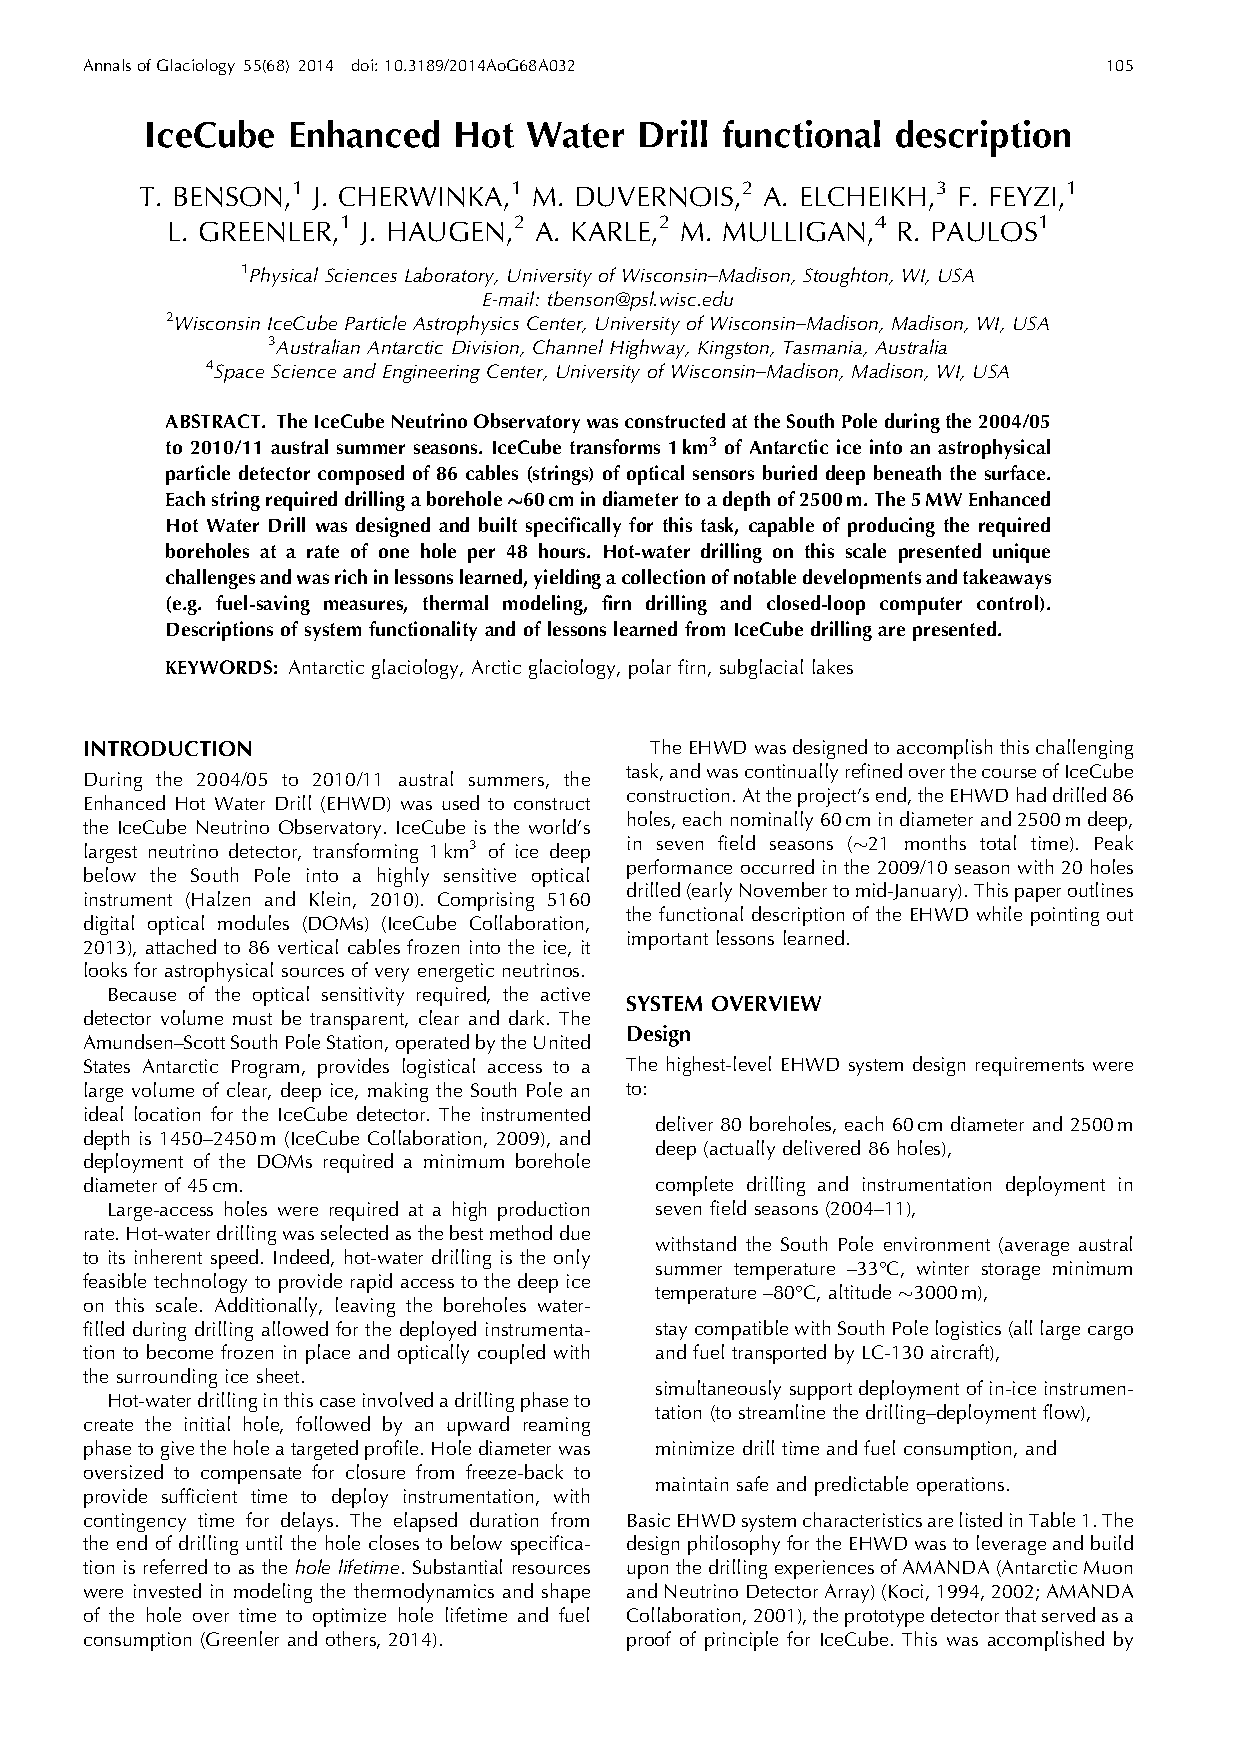
\includegraphics{ic/ic_drill.pdf}
    \caption[IceCube enhanced hot water drill]{The hole drilling part of the IceCube Enhanced Hot Water Drill, excluding the supply for hot, pressurized water. One can see the tower operations site above the hole and the hoses providing hot water and returning cooled water from the borehole back to the generators in a closed loop. From~\cite{Benson2014}.}
    \labfig{ic_drill}
\end{figure}

\subsection{The IceTop Surface Array}
In addition to the in-ice detector, IceCube has a surface air shower detector for cosmic-ray physics (see Section~\ref{cosmic_rays}), named IceTop. It was designed to study the cosmic-ray mass composition by correlating the energy it measures on the surface with the energy deposited by muons in the ice as measured by the in-ice detector~\sidecite{Abbasi2013}. The energy sensitivity range of IceTop is \SI{300}{\tera\eV} to \SI{1}{\exa\eV}~\sidecite{Aartsen2013a}.

\begin{marginfigure}
    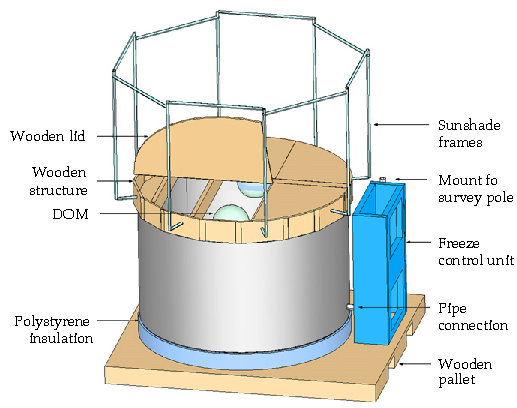
\includegraphics{ic/ic_icetop.pdf}
    \caption[IceTop detector]{IceTop surface Cherenkov detector tank. From~\cite{Abbasi2013}.}
    \labfig{ic_icetop}
\end{marginfigure}

The IceTop surface array consists of $2\times81$ ice-filled Cherenkov tanks. These are placed in pairs on the same hexagonal grid as the DOM strings for the in-ice array. Each tank is equipped with two standard IceCube DOMs (see Section~\ref{DOM})~\cite{Abbasi2013} which are operated at two different gain levels to increase the dynamic range.

Results from three years of IceTop data show good agreement between models describing the transition from galactic to extragalactic cosmic rays at energies above the knee. In these, the spectrum of lighter elements softens earlier towards higher energies compared to heavier elements. This is indeed reflected in the data~\sidecite{Aartsen2019}.

Furthermore, IceTop can be used to increase the purity astrophysical neutrino samples by vetoing muon events that mostly stem from cosmic-ray induced air showers, as opposed to muons created by neutrino interactions~\sidecite{Amin2021} (more details on background rejection will follow in Section~\ref{background}).

\subsection{Data Acquisition}\label{data_acquisition}
As noted above, only for locally coincident hits in multiple detectors the full waveforms are digitized by the DOMs. These are then sent to the IceCube Laboratory on the surface via the twisted-pair cable data link. In the laboratory all DOM data is ingested into the data acquisition system (DAQ). Hits throughout the detector are investigated by the system to establish common causality by temporal and sometimes spatial patterns. All hits for which common causality can be established form an `event'. The rate of these events varies seasonally with the atmospheric muon flux, with a median event rate of \SI{2.7}{\kilo\Hz} and a total data rate of \SI{1}{\tera\byte\per\day} (roughly \SI{100}{\mega\bit\per\second})~\cite{Aartsen2017}.

Satellite bandwidth is limited and costly. Therefore, further on-site software triggers reduce the data rate to \SI{15}{\percent} of the initial rate. These events are then transmitted via satellite to the IceCube data center at the University of Wisconsin-Madison for further analysis. The full event stream is also written to redundant disks, which are moved twice per year to Madison~\cite{Aartsen2017}.

\subsection{Time Synchronization}
Precise timing information is crucial to reconstruct an event (see Section~\ref{reconstruction}). For this reason, all DOMs need to be synced to a common clock. This is achieved by syncing the whole system to a Symmetricom ET6000 GPS receiver. The synchronization of individual DOMs is performed once per second, while data transfer is paused during the process (the calibration sequence takes $\lesssim$\SI{1.3}{\milli\second})~\sidecite{Abbasi2009}.

IceCube ensures temporal synchronicity with an algorithm called Reciprocal Active Pulsing (\texttt{RAPcal}): A bipolar pulse is initiated on the surface and sent to the DOM. The sender saves the local time when it sends the pulse and starts a timer. Upon reception down the string, the DOM also saves its current local time, saves the received pulse waveform, starts a timer, responds with a bipolar pulse of its own and stops the timer. Upon reception, the surface station stops its timer and requests the received pulse waveform and all timing information from the DOM.

With these six pieces of information---the two transmit timestamps, the two receive timestamps and both waveforms---a transformation from the GPS-synchronized surface to the local DOM time domain and vice versa can be calculated, with a precision of \SIrange{1}{2}{\ns}~\cite{Abbasi2009}.

\section{Angular Reconstruction}\label{reconstruction}

\begin{marginfigure}
    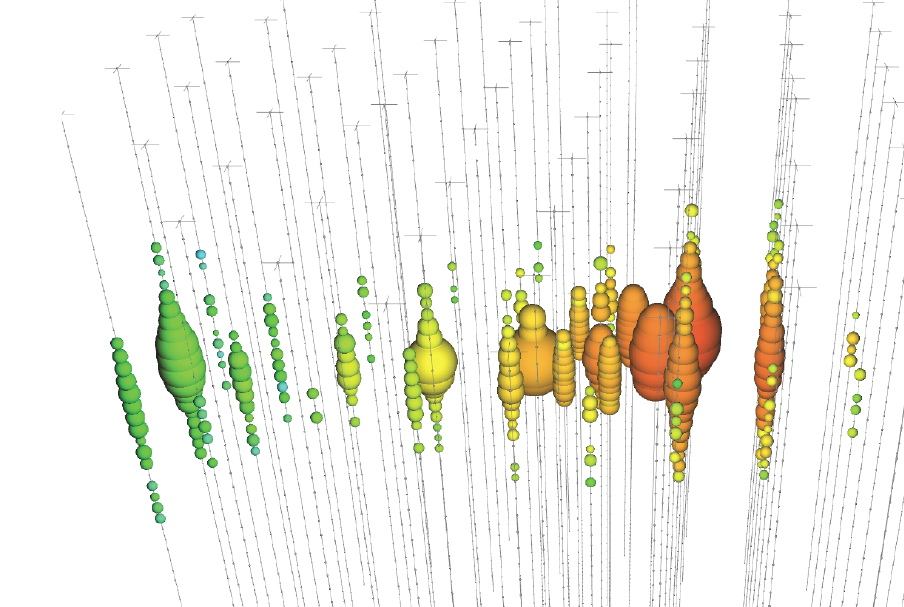
\includegraphics{ic/ic_track.png}
    \caption[Track event in IceCube]{Cascade event: The long track allows for good angular reconstruction, with high uncertainty on the event energy. From \url{masterclass.icecube.wisc.edu}.}
    \labfig{ic_track}
\end{marginfigure}
\begin{marginfigure}
    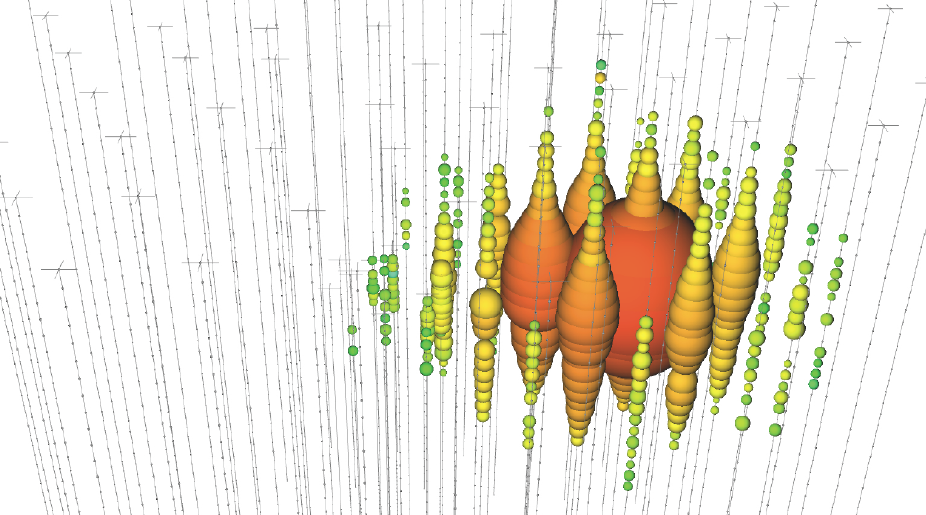
\includegraphics{ic/ic_cascade.png}
    \caption[Cascade event in IceCube]{Cascade event: The energy is fully contained in the detector, as the event is relatively isotropic. The angular uncertainty is quite large though. From \url{masterclass.icecube.wisc.edu}.}
    \labfig{ic_cascade}
\end{marginfigure}

The goal of IceCube reconstruction is twofold: Reconstructing the deposited neutrino energy, and reconstructing the neutrino arrival direction. With this in mind, one can sort the events seen by the detector broadly into two categories: Well-localized track events with poorly reconstructed energy, and cascade events with well-determined energy, but very imprecise origin.

\subsection{Event Types}\label{ic_event_types}

\begin{description}
    \item[Track Events] (Fig.~\ref{fig:ic_track}) are produced by secondary muons resulting from the charged-current interaction of muon neutrinos with the Antarctic glacial ice (see section~\ref{neutrinos_current}). The secondary muons leave tracks in the ice with a length on the order of kilometers. Muons with energies above \SI{\sim300}{\giga\eV} create tracks that exceed the detector length. In general, these allow for a good angular resolution, ranging from \SI{1}{\degree} for a \SI{1}{\TeV} muon to \SI{0.3}{\degree} for a \SI{1}{\peta\eV} muon~\sidecite{Abbasi2022}. The drawback is the large energy uncertainty of $0.25 \log{E_\mu}$ for a muon of energy $E_\mu$~\sidecite{Aartsen2014a}, as parts of the high-energy muon tracks lie outside the instrumented volume~\sidecite{Aartsen2017a}.

    \item[Cascade Events] (Fig.~\ref{fig:ic_cascade}) on the other hand are initiated by the charged-current interactions of $\nu_e$ and $\nu_\tau$, as well as by neutral-current interactions from neutrinos of all flavors. They are usually relatively isotropic and contained within the detector, as typical track lengths are of $\mathcal{O}(\SI{10}{\meter})$. Their relative isotropicity only allows for poor angular resolution (\SIrange{10}{15}{\degree}), but comparably good energy reconstruction ($\frac{\delta E}{E} \approx \SI{15}{\percent}$)~\cite{Aartsen2017a}.
\end{description}

As this thesis is concerned with the sources of high-energy astrophysical neutrinos and the angular resolution of track events allows for a better pointing accuracy compared to cascade events, the next section will focus on the angular reconstruction of the former.

\subsection{Likelihood Approach}
The main angular reconstruction algorithm for muon tracks used in IceCube is based on the work done for AMANDA. It employs a maximum-likelihood method~\sidecite{Ahrens2004}. This can be understood as follows: Given a set of unknown track parameters $\vec{a}$ and a set of experimentally determined values $\vec{x}$, what values of the unknown parameters $\vec{a}$ do maximize the probability of measuring the actually observed values $\vec{x}$?

This likelihood is denoted $\mathcal{L}(\vec{x}|\vec{a})$. If the components $x_i$ of $\vec{x}$ are independent, it can be expressed as

\begin{equation}
    \mathcal{L}(\vec{x}|\vec{a}) = \prod_i p(x_i|\vec{a}).
\end{equation}

Here, $p(x_i|\vec{a})$ is the probability density function (PDF) of measuring $x_i$ given a set of parameters $\vec{a}$. The reconstruction consists in obtaining the set of unknown track parameters $\vec{a}$ that maximizes the likelihood $\mathcal{L}$ (or, for technical reasons, minimizes $-\log{\mathcal{L}}$).

\subsection{Parametrization}

To simplify matters, we assume that we are dealing with a muon with maximum allowed speed ($\beta=1$), traveling along a track of infinite length. Furthermore, we neglect stochastic photon losses, which are mainly caused by impurities within the Antarctic ice (see below). The set of parameters $\vec{a}$ needed to describe the physical situation in the detector is visualized in Fig.~\ref{fig:ic_reco_cherenkov}: $\vec{a}$ = ($\vec{r_0}$, $E_0$, $t_0$, $\vec{p}$). It describes the trajectory of a muon located at position $\vec{r_0}$ with energy $E_0$ at time $t_0$, and traveling in the direction $\vec{p}$.

\begin{figure}[htb]
    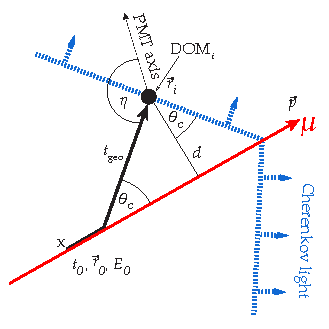
\includegraphics[width=0.6\textwidth]{ic/amanda_reco.pdf}
    \caption[Angular reconstruction in IceCube]{Parametrization for the angular muon reconstruction, describing the trajectory of a muon (red line) with energy $E_0$ that is in position $\vec{r_0}$ at time $t_0$, traveling towards direction $\vec{p}$. Cherenkov light from that muon is detected by a DOM at position $\vec{r_i}$ at distance $d$ to the trajectory with a light travel time $t_\text{geo}$. Adapted from~\cite{Ahrens2004}.}
    \labfig{ic_reco_cherenkov}
\end{figure}

So we are dealing with one time parameter, one energy parameter and positional parameters in 5 dimensions, where the vertex position $\vec{r}_0$ can be expressed in (x,y,z) and the muon direction $\vec{p}$ is usually described by two angles, zenith and azimuth\sidenote[][-40pt]{The zenith angle is the angle to a line vertical to the Earth, centered on the detector surface and pointing `southwards' (away from the Earth). An azimuth angle of \SI{90}{\degree} describes a particle traveling from North (prime meridian pointing towards Greenwich) to South, while a particle with an azimuth angle of \SI{0}{\degree} travels along the 90th Meridian from East to West.}. In the context of IceCube muon reconstruction, this parameter set $\vec{a}$ is known as the `track hypothesis'.

Now, a DOM in the detector at position $\vec{r}_i$ at a distance $d$ to the track can be hit by Cherenkov photons emitted by the muon traveling along the track with the Cherenkov angle $\theta_\text{C}$, arriving at an angle $\eta$ with respect to the PMT axis. Without scattering, the photon reaches the $\text{DOM}_i$ at the geometrical time $t_\text{geo}$, which can be expressed as

\begin{equation}
    t_\text{geo} = t_0 + \frac{|\vec{p}\cdot(\vec{r_i}-\vec{r_0})|+d\cdot \tan{\theta_\text{C}}}{c_0},
\end{equation}

with $c_0$ the vacuum speed of light. As this does not take scattering into account, it is useful to define a relative time of arrival, the time residual $t_\text{res} = t_\text{hit} - t_\text{geo}$. This is the additional time introduced by scattering as opposed to a Cherenkov photon traveling directly from the muon to the DOM\@.

To first order, the scattering does not loose light, but delays the photons. It is dominated by Mie scattering on impurities located within the ice. These impurities are thought to mainly comprise mineral dust, salt, acid droplets and soot by volcanic activity, all deposited by snow fall during the last 100,000 years~\sidecite{Abbasi2022a}.

As the position of the DOM is known, $t_\text{res}$ is the most significant observable for each DOM. We therefore simplify the $x_i$ in the likelihood's PDF to $t_{\text{res},i}$ and express $\vec{a}$ as a function of the individual DOM parameters: $\vec{a}= (d_i,\eta_i,\ldots)$, where $\eta_i$ is the angle to the DOM PMT axis (see Fig.~\ref{fig:ic_reco_cherenkov}).


\subsection{First (Single) Photoelectron Fit}
Matters can be simplified further. While the muon is traveling and emitting Cherenkov light, multiple photons can hit each DOM\@. One approximation is to only regard the first photon hitting an individual DOM, as it is usually less scattered than the average photon. If the reconstruction is using this simplification, it is called Single Photoelectron (SPE) fit. The likelihood function for this is\sidenote{As stated above, this already includes the reduction of $x_i$ to $t_{\text{res},i}$.}

\begin{equation}
    \mathcal{L}_\text{1st}(\vec{x}|\vec{a}) = \prod_i^\text{1st hits} p(t_{\text{res},i}|\vec{a}=d_i, \eta_i,\ldots),
\end{equation}

where the probability density function $p(t_{\text{res},i}|\vec{a})$ is obtained from simulations modeling the photon propagation through the Antarctic ice (this is necessary because the photon scatter needs to be accounted for). The simulation results are either stored in look-up tables or approximated by analytical functions~\cite{Ahrens2004}.

\subsection{Multi Photoelectron Fit}
A complication is that the first photon in a DOM detecting multiple photons tends to hit the DOM earlier than a photon detected by a DOM only registering this very photon. This is because more photon hits mean that the DOM is closer to the event, and therefore receives a higher signal---which means that the event is detected earlier on.

This complication leads to the Multi Photoelectron (MPE) fit. Here, the single-photon part of the likelihood is modified by the cumulative PDF (CDF), which is given time-integrating the photon arrival PDF from the $t_\text{res}$ to infinity:

\begin{equation}
    P(t_{\text{res},i}|\vec{a}) = \int^{\infty}_{t_{\text{res},i}}p(t|\vec{a})\,dt.
\end{equation}

Using this, the MPE likelihood is given as

\begin{equation}
    \mathcal{L}_\text{MPE} = \prod_i^\text{1st hits} p(t_{\text{res},i}|\vec{a}) \cdot N_i \cdot (1-P(t_{\text{res},i}|\vec{a}))^{N_i-1},
\end{equation}

where $N_i$ is the total number of photons recorded by $\text{DOM}_i$~\cite{Ahrens2004}. This is almost what is used in the angular reconstruction of the alerts IceCube distributes (see Section~\ref{ic_alerts}). The only difference is the PDF in question, which is described in the following Section~\ref{spline_mpe}.

\subsection{\texttt{SplineMPE} Reconstruction}\label{spline_mpe}
So far, nothing has been said about the photon arrival time PDF $p(t_\text{res}|\vec{a})$. The most straightforward approach is using a Gaussian distribution, which models the muon moving through the ice as plane wave of constant velocity. This can be enriched by assuming a more physically correct minimally ionizing muon track. When doing so, the PDF becomes a Gamma distribution of the form
\begin{equation}
    p(t_\text{res}) = \frac{\beta^\alpha t_\text{res}^{\alpha-1} e^{-\beta t_\text{res}}}{\Gamma(\alpha)},
\end{equation}
where $\alpha=\frac{d_\text{eff}}{\lambda}$, $\beta=\frac{1}{\tau} + \frac{c_m}{\lambda_\alpha}$. Here $\lambda$ is the scattering length, $\lambda_\alpha$ the absorption length, $c_m$ is the speed of light in a transparent medium and $\Gamma$ is the Gamma function. $d_\text{eff}$ is a modified version of the distance to the DOM $d$ that takes into account that the PMTs face downwards, and light from a track above a DOM needs to scatter around the DOM first (thus introducing an additional angle describing this delay). The scattering and absorption lengths $\lambda$ and $\lambda_a$, as well as the unspecified parameter $\tau$ have been determined by Monte Carlo simulations~\sidecite{Abbasi2021a}.

\texttt{SplineMPE} uses a more sophisticated PDF, as the Gamma PDF above assumes an optically homogenous medium. This is not the case for Antarctic ice. For this reason, a fitted ice model derived from measurements with the Flasher Board (see Section~\ref{DOM}) is used.

The basic idea is to create a large lookup table of simulated minimally ionizing muon tracks of infinite length with many different positions and orientations, i.e.\ high-dimensional histograms. A comprehensive lookup table of these simulations would be too large (hundreds of \unit{\giga\byte}) and numerically problematic due to empty bins or interpolation artifacts~\sidecite{Whitehorn2013}. To mitigate this, the histograms are normalized and interpolated with multidimensional basis splines. These splines then represent the photon arrival PDF dependent on the track vertex and orientation in the detector. They are defined by knots of fixed positions, so the PDF becomes
\begin{equation}
    p(t_\text{res}) = \sum_{i=1}^{T-k-1} w_i B_{i,k}(t_\text{res},\vec{a}, \kappa).
\end{equation}

Here $T$ is the total number of knot positions, $B$ is the $i$-th basis spline of order $k$, $\vec{a}$ again describes the track, and $\kappa$ denotes the parameters of the ice model~\cite{Whitehorn2013}.

\subsection{\texttt{Millipede} Reconstruction}\label{millipede}

\begin{marginfigure}
    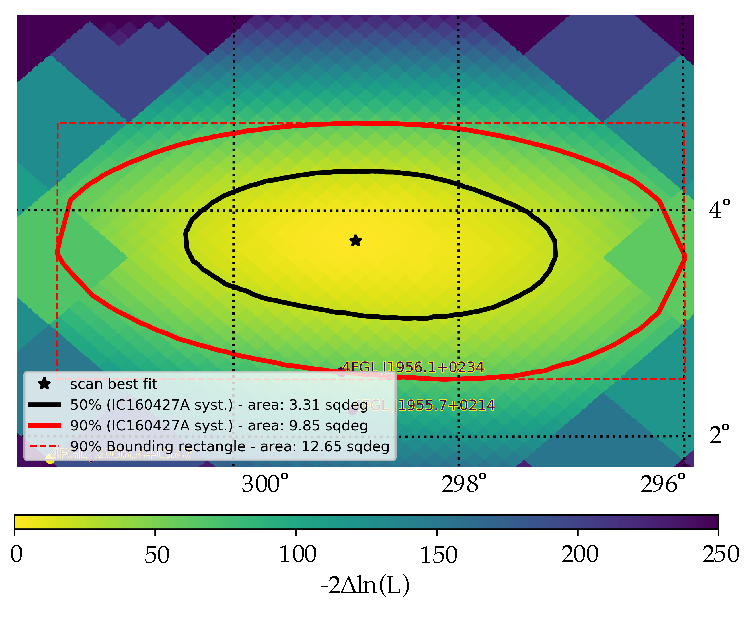
\includegraphics[width=1\textwidth]{ic/ic_millipede_IC221124A.pdf}
    \caption[\texttt{Millipede} reconstruction of \emph{IC221124A}]{\texttt{Millipede} reconstruction of \emph{IC221124A}.}
    \labfig{ic_millipede}
\end{marginfigure}


High-energy neutrino events that pass the realtime alert selection criteria (see Section~\ref{ic_alert_program}) are subjected to a more sophisticated algorithm, which uses the information from all the detected photons. This algorithm is dubbed \texttt{Millipede}. Due to its high demand of computational resources it is only run for selected events at the IceCube data center in Madison.

This reconstruction consists of a maximum likelihood scan covering the whole sky. To allow scanning, the sky is pixelated into grids of increasing resolution following the Hierarchical Equal Area isoLatitude Pixelation (\texttt{HEALPix}) scheme~\sidecite{Gorski2005}. Each pixel of a specific resolution covers the same area on the sky. For each scanned pixel, the muon direction is fixed to originate from that sky location.

For this fixed direction, the likelihood of the deposited energy resulting from the best fit and the neutrino interaction vertex in the detector are then computed. Pixels near the likelihood maximum are then scanned again with a finer \texttt{HEALPix} resolution. This procedure ultimately results in a likelihood map of the sky with increasing granularity towards the global maximum~\sidecite{Abbasi2023}.

To compute the \SI{50}{\percent} and \SI{90}{\percent} confidence level uncertainty contours, Monte Carlo resimulations from the high-energy neutrino event \emph{IC160427A} are used. For this event, Pan-STARRS found a possible counterpart, \emph{PS16cgx}\sidenote{Spectroscopic follow-up revealed that this event was either an SN Ic, which would be compatible with neutrino production, or---more likely---an SN Ia, which would exclude it as a neutrino source~\cite{Kankare2019}.}~\sidecite{Kankare2019}.

In the resimulations, the systematic parameters of the Antarctic ice used to model photon propagation were varied. Additionally, the simulated directions and energies were varied, with cuts to ensure that the light deposition of the resimulations resembled the original event (\SI{\pm2}{\degree} in direction, \SI{\pm20}{\percent} in deposited charge).

Each resimulated event was fit with \texttt{Millipede}. The distribution of differences between the best-fit likelihood and the ground truth of the simulated event were then employed to convert the change in log-likelihood over the map into a confidence level.

Due to the systematic uncertainties involved, Wilk's theorem does not apply here. To account for this fact, the contours derived for individual events (which make use of the theorem) are scaled up with correction values obtained from the resimulations of \emph{IC160427A}. Then, all pixels that satisfy $\log \mathcal{L}_\text{min}-\log \mathcal{L}_\text{pixel} = -11.3$ $(-32.1)$ form the \SI{50}{\percent} (\SI{90}{\percent}) error contours. Currently, these correction values are 22.2 and 64.2 for the \SI{50}{\percent} and \SI{90}{\percent} uncertainty contours~\sidecite{Gualda2021}. In Fig.~\ref{fig:ic_millipede} these contours are displayed for an example event. The black line shows the \SI{50}{\percent} uncertainty region, while the red line shows the \SI{90}{\percent} area.

However, resimulations of newer high-energy neutrino events have shown that the method of scaling up the errors with correction values obtained from resimulating \emph{IC160427A} does in some cases not faithfully capture the errors of those newer resimulations: They are sometimes under- and sometimes overestimated, depending on the topography of the event. For details on this, see~\cite{Gualda2021}.

\section{The Realtime Alert Program}\label{ic_alert_program}
Since 2016, IceCube hosts a realtime alert program, providing the astrophysical community with low-latency and high-quality astrophysical neutrino alerts~\cite{Aartsen2017a}. This program saw a major revision in 2019, when two new alert streams, named `Gold' and `Bronze', were created~\sidecite{Blaufuss2019}. As these were designed based on cuts reducing the IceCube background, one needs to understand the background contamination first.

\subsection{Background}\label{background}

When searching for the sources of astrophysical neutrinos, there are two major sources of background events in the IceCube detector. Both stem from secondary cosmic-ray particles from the Earth's atmosphere.

\begin{figure}[htb]
    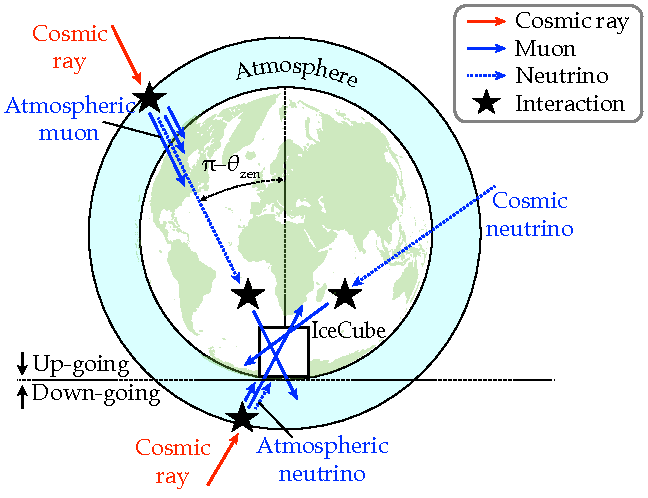
\includegraphics[width=0.8\textwidth]{ic/ic_background.pdf}
    \caption[Background events]{Background events in the detector. Cosmic rays hit the atmosphere around the globe and produce muons (solid blue arrows), as well as neutrinos (dashed blue arrows). When constraining to \textit{up-going} events from the northern hemisphere, the detector is shielded from atmospheric muons, but not atmospheric neutrinos, as these can traverse the Earth. Adapted from~\cite{Ahlers2018a}.}
    \labfig{ic_background}
\end{figure}

\begin{marginfigure}
    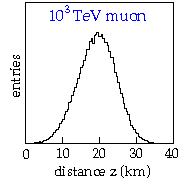
\includegraphics[width=0.8\textwidth]{ic/ic_muon_free_path.pdf}
    \caption[Muon free path in ice]{Free path length for \SI{1}{\peta\eV} muons in ice. The mean free path in ice is slightly longer than in rock. Adapted from~\cite{Chirkin2004}.}
    \labfig{ic_muon_free_path}
\end{marginfigure}

\begin{description}
    \item[Atmospheric Muons] are created by cosmic rays hitting the atmosphere. One can efficiently filter this background by restricting the analysis to \textit{up-going} muon tracks. These are tracks that come from the bottom of the detector, i.e.\ the northern hemisphere. Atmospheric muons stemming from cosmic-ray events in the northern hemisphere are filtered out by the Earth's core (see Fig.~\ref{fig:ic_background}), as the mean free path of muons within the Earth is much smaller~\sidecite{Chirkin2004} than the distance they have to cross (see Fig.~\ref{fig:ic_muon_free_path}). Note that due to light scattering within the ice, some down-going tracks can be misclassified as up-going~\sidecite{Ahlers2018a}.

          One complication here stems from the fact that the Earth starts to become opaque for neutrinos of higher energies. Studies interested in \si{\peta\eV} neutrinos therefore must deal with the fact that these get the more suppressed the longer their path through the Earth is. For example, a \SI{1}{\peta\eV} neutrino with a zenith angle of \SI{140}{\degree} is absorbed with \SI{90}{\percent} probability~\sidecite{Aartsen2017c}.
          \pagebreak

          %   \begin{figure}[htb]
          %       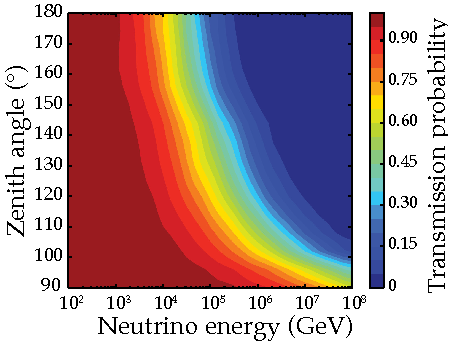
\includegraphics[width=0.5\textwidth]{ic/ic_absorption_earth.pdf}
          %       \caption[Neutrino absorption in the Earth]{Neutrino transmission probability through the Earth. The longer the distance traveled (higher zenith angles) and the higher the neutrino energy, the more likely is absorption. From~\cite{Aartsen2017c}.}
          %       \labfig{ic_absorption_earth}
          %   \end{figure}
          \begin{marginfigure}
              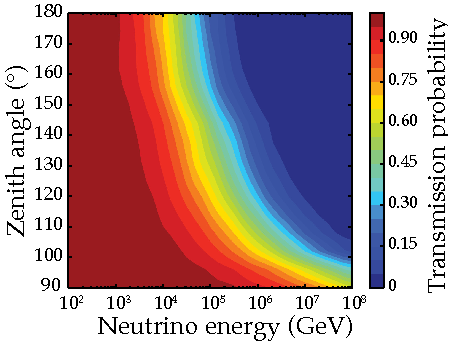
\includegraphics{ic/ic_absorption_earth.pdf}
              \caption[Neutrino absorption in the Earth]{Neutrino transmission probability through the Earth. The longer the distance traveled (higher zenith angles) and the higher the neutrino energy, the more likely is absorption. Adapted from~\cite{Aartsen2017c}.}
              \labfig{ic_absorption_earth}
          \end{marginfigure}
    \item[Atmospheric Neutrinos] also stem from cosmic-ray induced air showers. These cannot be suppressed by directional cuts, creating an irreducible background: When atmospheric neutrinos cross the Earth and interact with the matter close to the detector, they can produce muons indistinguishable from muons created by `proper' cosmic neutrinos~\cite{Ahlers2018a}.
          \begin{marginfigure}
              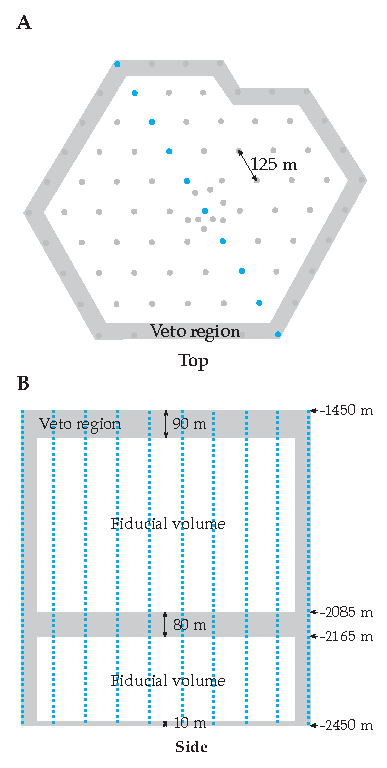
\includegraphics{ic/ic_HESE_veto.pdf}
              \caption[HESE veto regions]{High-energy starting events veto regions. The strings marked in blue in the top-down view at the top (A) show the location of the side view, displayed at the bottom (B). Adapted from~\cite{Aartsen2013}.}
              \labfig{ic_hese_veto}
          \end{marginfigure}
\end{description}

\subsection{Event Selection}\label{ic_event_selection}

Gold and Bronze alerts are drawn from three different selection schemes, originally designed to cater to different science goals. These are High Energy Starting Events (HESE)~\sidecite{Abbasi2021}, Extremely High Energy (EHE) events~\sidecite{Aartsen2016} and Gamma-Ray Follow Up (GFU) events~\sidecite{gfu2016}.

\begin{description}

    \item[HESE] are events that start within the detector. This is guaranteed by using the outer regions of the detector as a veto region, in which (almost) no Cherenkov light must be detected~\cite{Aartsen2013}. The sizes of those regions can be seen in Fig.~\ref{fig:ic_hese_veto}. The majority of HESE events are cascade-type events and therefore not well suited for observational follow-up due to their poor angular reconstruction. Because of this drawback, additional cuts are applied: At least 6000 photoelectrons are required, the reconstruction must favor a track interpretation of the event, and the reconstructed track length must be at least \SI{200}{\meter}~\cite{Abbasi2023}. Note that the selection criteria used in the Gold and Bronze HESE selection are slightly different from those in the original paper cited above.

    \item[EHE] aims at neutrino energies of \SIrange{0.5}{10}{\peta\eV}. To reject atmospheric background events, a two-dimensional cut depending on the reconstructed zenith angle and the log of detected photoelectrons is applied. Additionally, a $\chi^2$-based goodness-of-fit cut is applied to select track-like events with good reconstructions~\cite{Abbasi2023}.

    \item[GFU] events are selected based on a boosted decision tree trained to identify through-going (as opposed to `starting') track events with astrophysical origin. Energy cuts are applied: Northern hemisphere events are selected based on their reconstructed muon energies, while events from the southern hemisphere are selected based on the total photoelectron charge deposited in the detector.
\end{description}

The cuts from all three event pools are gauged to achieve two different average values of signalness, which is a proxy for the probability that the event is of astrophysical origin~\cite{Abbasi2023}. It is defined as
\begin{definition}\label{signalness_def}
    $\text{Signalness}(E,\theta_\text{zen}) = \frac{N_\text{signal}(E,\theta_\text{zen})}{N_\text{signal}(E,\theta_\text{zen})+N_\text{background}(E,\theta_\text{zen})}$
\end{definition}
Here $E$ is the reconstructed neutrino energy, and $N_\text{signal}(E,\theta_\text{zen})$ and $N_\text{background}(E,\theta_\text{zen})$ are the number of signal and background events at zenith angle $\theta_\text{zen}$ above energy $E$ as determined by simulations~\cite{Abbasi2023}.

The cuts on the individual event selections are tuned to ensure that \textit{Gold} alerts on average have a signalness of \SI{50}{\percent}, and \textit{Bronze} alerts have an average signalness of \SI{30}{\percent}.

\subsection{Alert Distribution} \label{ic_alerts}
All events that pass a first stage of filtering are sent to the IceCube data center (see Section~\ref{data_acquisition}) via Iridium satellite to minimize latency. There, their signalness is computed. After this, they are globally distributed with the General Coordinates Network\sidenote{\url{https://gcn.nasa.gov/}} (GCN) in the form of GCN Notices.

Each notice contains the discovery time, a unique event number, the reconstructed direction in right ascension (RA) and declination (Dec) of the candidate neutrino computed by \texttt{SplineMPE} (see Section~\ref{spline_mpe}), a statistical error for the direction, the reconstructed neutrino energy, the signalness and the false alarm rate~\cite{Blaufuss2019}.

\begin{marginfigure}
    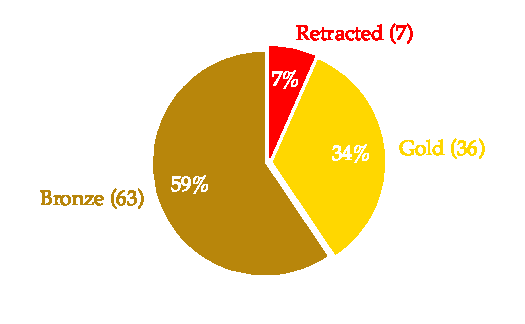
\includegraphics{ic/ic_he_alert_overview.pdf}
    \caption[IceCube alert overview]{High-energy neutrino alerts issued by IceCube since start of the new alert stream in June 2019.}
    \labfig{ic_he_alert_overview}
\end{marginfigure}

This information is later appended by \texttt{Millipede}, a computationally more demanding, but more sophisticated reconstruction (see Section~\ref{millipede}). The results of these reconstructions (i.e.\ the angular uncertainty) are typically distributed a few hours after the initial notice in the form of a GCN circular, and an updated GCN notice~\cite{Blaufuss2019}.

As of March 2023, a total of 106 events have been distributed in this format, with 7 later being retracted. Since the start of the Gold and Bronze alert streams in June 2019, this amounts to 2.2 non-retracted alerts per month\sidenote{This is quite close to the 2.5 alerts per month predicted in~\cite{Blaufuss2019}.} (0.8 Gold alerts, 1.4 Bronze alerts). For a full list of all high-energy neutrino alerts issued by IceCube, not only those since introduction of the Gold and Bronze format, see~\cite{Abbasi2023}.

If the neutrino is most likely astrophysical and its origin reasonably well pinpointed, one can scan the sky localization with a telescope and look for potential sources of the neutrino. But where to obtain optical images from? The telescope used for this, the Zwicky Transient Facility, will be described in Chapter~\ref{ztf}.



